\documentclass[10pt,A4paper]{report}
\usepackage{amsmath}
\usepackage{microtype}	% Font improvement for pdflatex.
\usepackage{pgf}
\usepackage{tikz}
\usepackage{verbatim}
\usepackage{url}
\usepackage{hyperref}	% Clickable links to figures, references and urls.
\usepackage{float}		% Floating figure placement.
\usepackage{graphicx}
\usepackage{subfigure}

% Listings for wrapping code.
\usepackage{listings}
\lstset{breaklines=true}
\lstset{basicstyle=\small\ttfamily}

% Figures folder.
\graphicspath{{Figures/}}

%Chapter 1 Introduction to FDTD
%1. 1D Equations
%2. 1D simple wave propagation
%3. Additive source, Stability, significance of Sc
%4. Boundary conditions
%Chapter 2 Dispersive Media
%5. 1D scatterer using Drude, epsilon=2
%6. 2D dispersive media, cylinder problem from Sadiku using Drude
%Chapter 3 Metamaterial Modelling using Dispersive Drude Model
%7. 1D DNG slab
%8. 2D DNG slab
%Chapter 4 FDTD Modelling of Lossless Cylindrical Cloak
%9. 2D FDTD implementation on Matlab
%10. 2D FDTD implementation on C++
%Chapter 5 GPU implementation of Lossless Cylindrical Cloak
%11. GPU considerations
%12. Implementation details
%13. Performance Analysis
%Conclusion

\begin{document}

\pagenumbering{roman}

% Title Page.
\input{FDTDTitle}

\begin{center}
\copyright Copyright\\[0.2in]
by\\[0.2in]
Attique Dawood\\[0.2in]
2012
\end{center}

\include{FDTDCertification}

\tableofcontents
\addtocontents{toc}{~\hfill\textbf{Page}\par}	% Ref: http://texblog.org/2011/09/09/10-ways-to-customize-tocloflot/
\listoffigures

\begin{abstract}
The Finite Difference Time-Domain method is a differential numerical technique for solving electromagnetic wave scattering problems. In order to model metamaterials with negative refractive index the standard algorithm is modified as implementation of the Drude dispersion model. Suitable values of plasma frequency ($\omega_p$) are chosen to model the metamaterial cloaking structure following the treatment of~\cite{Radial-Zhao}. The lossless case of electromagnetic cloak is implemented using a graphics processing unit (GPU). Simulation performance on Matlab, C++ and GPU is analysed.
\end{abstract}

\pagenumbering{arabic}

% Introductory chapter.
\chapter{Introduction}
\section{Metamaterials}
The concept of metamaterials\index{metamaterial} was originally put forward by a Russian physicist Victor Veselago\index{Victor, Veselago} in the late 60's~\cite{Newelectronics-Metamaterial}. Metametrials are essentially substances with negative values of permeability and permittivity\index{DNG}. These are artificially manufactured with certain structural geometry. Electromagnetic waves passing through these metamaterials will act differently compared to naturally occurring materials. The behaviour of these metamaterials can change with frequency of incident EM wave and may exhibit negative values of permittivity and permeability under certain conditions. Some applications of metamaterials are perfect lens\index{perfect lens}, invisibility cloak\index{cloak} and novel antenna designs.
\section{Modelling Techniques}
Metamaterials can be modelled using analytical\index{analytical technique} or numerical\index{numerical technique} techniques. For problems with simple geometry and symmetry analytical methods give exact solution. For complex structures and irregular geometries, numerical techniques can be applied. Numerical techniques in electromagnetics are generally classified as either differential or integral. Examples of integral techniques are method of moment (MoM)\index{method of moment (MoM)} and finite element method (FEM)\index{finite element method (FEM)}, whereas, finite difference time--domain (FDTD)\index{FDTD} is a differential technique.
\section{FDTD Modelling}
Integral techniques usually involve solving for unknowns in the problem domain. The number of unknowns determine the computational time required. On the other hand, FDTD\index{FDTD} is a brute force method that requires the whole problem domain to be discretised and stored in computer memory. Thus, the amount of computer memory is a constraint in the case of FDTD\index{FDTD}. Conceptually, FDTD\index{FDTD} is easier compared to integral methods.
\section{FDTD on Modern Hardware}
In recent times computer memory has become extremely cheap and a large number of complex problems can be readily and easily modelled using FDTD\index{FDTD}. Moreover, the recent advent of multi--core CPUs\index{CPU} (central processing unit) favour methods and algorithms that can take advantage of parallel processing. Since, FDTD\index{FDTD} is a data parallel algorithm it is ideal in such a scenario.

In more recent times, GPUs\index{GPU} (graphics processing units) with general purpose computing capabilities have arrived on the scene. These GPGPUs\index{GPU!general purpose (GPGPU)} are in the order of 5--20 times faster than contemporary CPUs\index{CPU} and are heavily multi--threaded. The goal of this thesis is to implement the classical cylindrical cloak\index{cloak} on GPU\index{GPU} using the FDTD\index{FDTD} method proposed in~\cite{Radial-Zhao}.

%\chapter{FDTD Modelling of Metamaterials}
\chapter{Introduction to Finite Difference Time--Domain Technique}
\section{The Yee Algorithm}
The original algorithm was\index{Yee algorithm} proposed by K. S. Yee\index{Yee, K. S.} in 1966~\cite{Yee1966}. The derivatives in Faraday's Law\index{Faraday's Law} and Ampere's Law\index{Ampere's Law} are replaced with difference equations. The whole problem space is discretised and divided into cells such that electric and magnetic fields are staggered at half spatial steps in unit cell. By advancing the simulation in time, future values of electric and magnetic field components are computed using past values. This chapter gives provides a brief treatment of FDTD\index{FDTD} in 1D and 2D. Wave propagation in free space and with a homogeneous scatterer are discussed using conventional and dispersive FDTD\index{FDTD!dispersive} methods.
\section{FDTD Update Equations in One Dimension (1D)}
Faraday's Law\index{Faraday's Law} and Ampere's Law\index{Ampere's Law} in differential form are given by:
\begin{equation}
\centering
\nabla \times \textbf{E} = - \dfrac{\partial \textbf{B}}{\partial t}
\label{Faraday's Law}
\end{equation}
\begin{equation}
\centering
\nabla \times \textbf{H} = \dfrac{\partial \textbf{D}}{\partial t}
\label{Ampere's Law}
\end{equation}
Assume electric field only has $x$--component, that is $E_x$, and magnetic field only has $y$--component $H_y$. The curl of electric field can be expanded as:
\begin{equation}
\centering
\nabla \times \textbf{E} = - \mu \dfrac{\partial H_y}{\partial t} \hat{y} = \left| \begin{array}{ccc} \hat{x} & \hat{y} & \hat{z} \\ \frac{\partial}{\partial x} & \frac{\partial}{\partial y} & \frac{\partial}{\partial z} \\ E_x & 0 & 0 \end{array} \right| = \dfrac{\partial E_x}{\partial z} \hat{y}
\label{Faraday's Law-Curl-Expansion}
\end{equation}
Similarly, the curl of magnetic field can be written as:
\begin{equation}
\centering
\nabla \times \textbf{H} = \epsilon \dfrac{\partial E_x}{\partial t} \hat{x} = \left| \begin{array}{ccc} \hat{x} & \hat{y} & \hat{z} \\ \frac{\partial}{\partial x} & \frac{\partial}{\partial y} & \frac{\partial}{\partial z} \\ 0 & H_y & 0 \end{array} \right| = - \dfrac{\partial H_y}{\partial z} \hat{x}
\label{Ampere's Law-Curl-Expansion}
\end{equation}
Rearranging terms,
\begin{equation}
\centering
\dfrac{\partial H_y}{\partial t} = - \dfrac{1}{\mu} \dfrac{\partial E_x}{\partial z}
\label{Faraday's Law-Curl-Expansion-1D}
\end{equation}
\begin{equation}
\centering
\dfrac{\partial E_x}{\partial t} = - \dfrac{1}{\epsilon} \dfrac{\partial H_y}{\partial z}
\label{Ampere's Law-Curl-Expansion-1D}
\end{equation}
These two scalar equations drive the FDTD\index{FDTD} algorithm. First, magnetic field is calculated using equation~\ref{Faraday's Law-Curl-Expansion-1D} and then electric field (equation~\ref{Ampere's Law-Curl-Expansion-1D}) is calculated from the magnetic field obtained in~\ref{Faraday's Law-Curl-Expansion-1D}. Electric and magnetic fields are staggered at half time steps. Similarly, magnetic and electric fields in space are also spaced at half spatial steps. The algorithm is normally referred to as a leap--frog scheme\index{leap--frog}.
\begin{figure}[here]
\centering
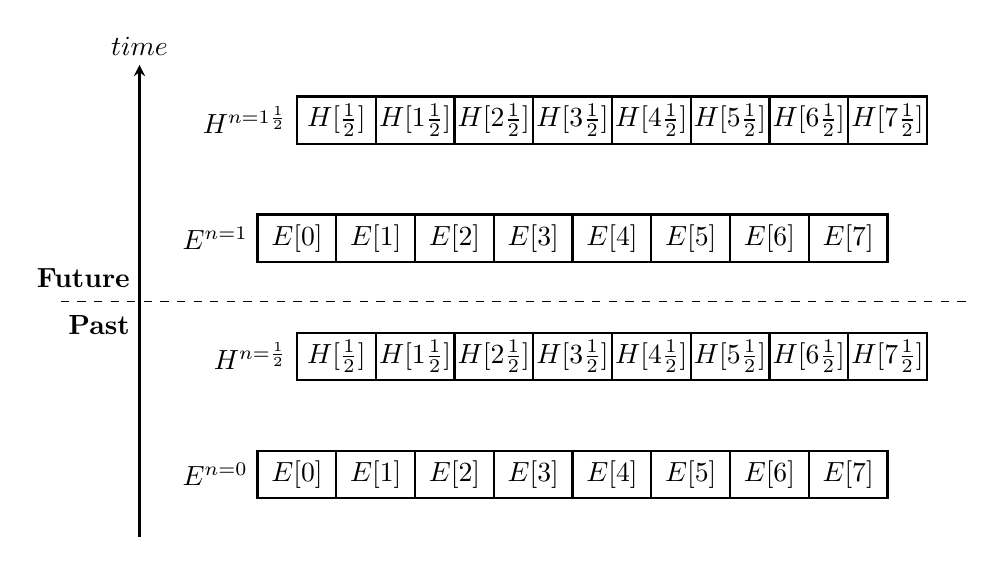
\begin{tikzpicture}
	\def\XD{0cm}
	\def\YD{0cm}
	\coordinate[label=left:$E^{n=0}$] (E0) at (\XD,\YD+0.3cm);
	\foreach \x in {0.0cm, 1.0cm, 2.0cm, 3.0cm, 4.0cm, 5.0cm, 6.0cm, 7.0cm}
		\draw[thick] (\XD+\x, \YD+0cm) rectangle (\XD+\x+1.0cm, \YD+0.6cm);
	\foreach \x/\y in {0.0cm/0, 1.0cm/1, 2.0cm/2, 3.0cm/3, 4.0cm/4, 5.0cm/5, 6.0cm/6, 7.0cm/7}
		\draw (\XD+\x+0.5cm,\YD+0.3cm) node {$E[\y]$};
	
	\def\XD{0.5cm}
	\def\YD{1.5cm}
	\coordinate[label=left:$H^{n=\frac{1}{2}}$] (H1/2) at (\XD,\YD+0.3cm);
	\foreach \x in {0.0cm, 1.0cm, 2.0cm, 3.0cm, 4.0cm, 5.0cm, 6.0cm, 7.0cm}
		\draw[thick] (\XD+\x, \YD+0cm) rectangle (\XD+\x+1.0cm, \YD+0.6cm);
	\foreach \x/\y in {0.0cm/\frac{1}{2}, 1.0cm/1\frac{1}{2}, 2.0cm/2\frac{1}{2}, 3.0cm/3\frac{1}{2}, 4.0cm/4\frac{1}{2}, 5.0cm/5\frac{1}{2}, 6.0cm/6\frac{1}{2}, 7.0cm/7\frac{1}{2}}
		\draw (\XD+\x+0.5cm,\YD+0.3cm) node {$H[\y]$};

	\draw[dashed] (-2.5cm,2.5cm) -- (9.0cm,2.5cm);

	\def\XD{0cm}
	\def\YD{3cm}
	\coordinate[label=left:$E^{n=1}$] (E1) at (\XD,\YD+0.3cm);
	\foreach \x in {0.0cm, 1.0cm, 2.0cm, 3.0cm, 4.0cm, 5.0cm, 6.0cm, 7.0cm}
		\draw[thick] (\XD+\x, \YD+0cm) rectangle (\XD+\x+1.0cm, \YD+0.6cm);
	\foreach \x/\y in {0.0cm/0, 1.0cm/1, 2.0cm/2, 3.0cm/3, 4.0cm/4, 5.0cm/5, 6.0cm/6, 7.0cm/7}
		\draw (\XD+\x+0.5cm,\YD+0.3cm) node {$E[\y]$};

	\def\XD{0.5cm}
	\def\YD{4.5cm}
	\coordinate[label=left:$H^{n=1\frac{1}{2}}$] (H11/2) at (\XD,\YD+0.3cm);
	\foreach \x in {0.0cm, 1.0cm, 2.0cm, 3.0cm, 4.0cm, 5.0cm, 6.0cm, 7.0cm}
		\draw[thick] (\XD+\x, \YD+0cm) rectangle (\XD+\x+1.0cm, \YD+0.6cm);
	\foreach \x/\y in {0.0cm/\frac{1}{2}, 1.0cm/1\frac{1}{2}, 2.0cm/2\frac{1}{2}, 3.0cm/3\frac{1}{2}, 4.0cm/4\frac{1}{2}, 5.0cm/5\frac{1}{2}, 6.0cm/6\frac{1}{2}, 7.0cm/7\frac{1}{2}}
		\draw (\XD+\x+0.5cm,\YD+0.3cm) node {$H[\y]$};


	\draw[thick, ->, >=stealth] (-1.5cm, -0.5cm) -- (-1.5cm, 5.5cm);
	\coordinate[label=above:$time$] (time) at (-1.5cm,5.5cm);
	\coordinate[label=left:\textbf{Past}] (Past) at (-1.5cm,2.2cm);
	\coordinate[label=left:\textbf{Future}] (Future) at (-1.5cm,2.8cm);

\end{tikzpicture}
\caption{FDTD leap--frog\index{leap--frog} scheme to update future fields from past fields}
\label{FDTD-LeapFrog}
\end{figure}
By examining equations~\ref{Faraday's Law-Curl-Expansion-1D} and \ref{Ampere's Law-Curl-Expansion-1D} it can be intuitively observed that a wave with $E_x$ and $H_y$ components will propagate in $\hat{z}$ direction and space derivatives with respect to $z$ indicate variation of electric and magnetic fields in space along $z$--axis.

These equations need to be discretised before they can be implemented as a computer simulation. Both the time and space derivatives are discretised to obtain difference equations. The difference equations for space and time derivatives use central difference\index{central difference} scheme and expressed as,
\begin{equation}
\centering
\dfrac{\partial F^n(x)}{\partial t} \equiv \dfrac{F^{n+\frac{1}{2}}(x)-F^{n-\frac{1}{2}}(x)}{\Delta t}
\label{central-difference-time}
\end{equation}
\begin{equation}
\centering
\dfrac{\partial F^n(x)}{\partial x} \equiv \dfrac{F^n(x+\frac{1}{2})-F^n(x-\frac{1}{2})}{\Delta x}
\label{central-difference-space}
\end{equation}
Following the treatment in chapter 3 of~\cite{JBSchneiderUFDTD}, electric and magnetic fields as functions of time and space can be written as,
\begin{equation}
\centering
H_y (z,t)=H_y (k\Delta _z,n\Delta _t)=H^n_y[k]
\label{Hy-of-z_and_t}
\end{equation}
\begin{equation}
\centering
E_x (z,t)=E_x (k\Delta _z,n\Delta _t)=E^n_x[k]
\label{Ex-of-z_and_t}
\end{equation}
The final equations for electric and magnetic fields driving the FDTD algorithm are\index{FDTD!update equations}
\begin{equation}
\centering
H^{n+\frac{1}{2}}_y \left[k+\frac{1}{2}\right]=H^{n-\frac{1}{2}}_y \left[k+\frac{1}{2}\right] + \dfrac{\Delta t}{\mu \Delta x} \left( E^{n}_x \left[k\right] - E^{n}_x \left[k+1\right] \right)
\label{Hy-1D-Simple-FDTD-Driver}
\end{equation}
\begin{equation}
\centering
E^{n+1}_x \left[k\right]=E^{n}_x \left[k\right] + \dfrac{\Delta t}{\epsilon \Delta x} \left( H^{n+\frac{1}{2}}_y \left[k-\frac{1}{2}\right] - H^{n+\frac{1}{2}}_y \left[k+\frac{1}{2}\right] \right)
\label{Ex-1D-Simple-FDTD-Driver}
\end{equation}
The FDTD\index{FDTD} code for this 1D simulation is given in appendix \ref{App:1DFDTDFreeSpaceMatlab} and uses first order absorbing boundary condition (ABC)\index{boundary condition!absorbing (ABC)}.
\section{Stability and Accuracy}
\subsection{Courant Stability Criterion}
Stability of the FDTD\index{FDTD} method is governed by the temporal time step $\Delta t$. If it is too large then the simulation would become unstable. In FDTD\index{FDTD} the fields exist at discrete locations. In one iteration or temporal step, energy should not propagate any further than the neighbouring field or node. This is known as the Courant Stability Criterion\index{Courant stability criterion} and is expressed as,
\begin{equation}
\centering
c \Delta t \leq \left[ \dfrac{1}{\Delta x^2} + \dfrac{1}{\Delta y^2} + \dfrac{1}{\Delta z^2} \right]^{-\frac{1}{2}}
\label{Courant-Stability-Criterion}
\end{equation}
For the case where spatial differentials are equal (denoted by $\delta$), this reduces to,
\begin{equation}
\centering
S_c = \dfrac{c \Delta t}{\delta} \leq 1
\label{Courant-Stability-Criterion-Equal-Differentials}
\end{equation}
Here $S_c$ is known as the Courant number\index{Courant number ($S_c$)}. It should be less than unity in order for a stable solution.
\begin{figure}[htb]
\centering
\mbox{\subfigure[$S_c = 1$]{\includegraphics[scale=0.375, trim=3.75cm 8.75cm 4.5cm 9.25cm, clip]{Figures/FigCh02_Stable1DFDTD.pdf}}\quad\subfigure[$S_c = 1.1$]{\includegraphics[scale=0.375, trim=3.75cm 8.75cm 4.5cm 9.25cm, clip]{Figures/FigCh02_Unstable1DFDTD.pdf}}}
\caption{$S_c$ and stability of FDTD}
\label{Unstable-FDTD}
\end{figure}
\subsection{Courant Number as Scaling Factor}
In one time step ($\Delta t$) the amount of distance travelled by an electromagnetic wave (in cells) is equal to Courant number. Since $S_c$ cannot be greater than unity, an EM wave can only travel one cell or $\Delta$ during one time stepping of algorithm. Simulations with values of $S_c$ close to unity can rapidly become unstable in the presence of an obstacle or scatterer. Smaller values of $S_c$ will result in better stability but the trade--off is an increase in simulation time.
\subsection{Wavelength and Cell Size}
The size of wavelength should be considerably greater than minimum spatial step. Normally wavelength is taken to be at least ten times the size of a single cell~\cite{Taflove2000}. It makes sense that there shouldn't be too much fluctuations between two spatial steps and wavelength should be spread over a reasonable number of cells. Figure~\ref{Pulsewidth-comparison} shows different sizes of Gaussian pulses\index{source!Gaussian pulse} in a 1D simulation. Decreasing pulse width below 10 cells results in noticeable fluctuations and this can result in inaccurate results.
\begin{figure}[htb]
%\centerline{\includegraphics[]{GPGPU}}
\centering
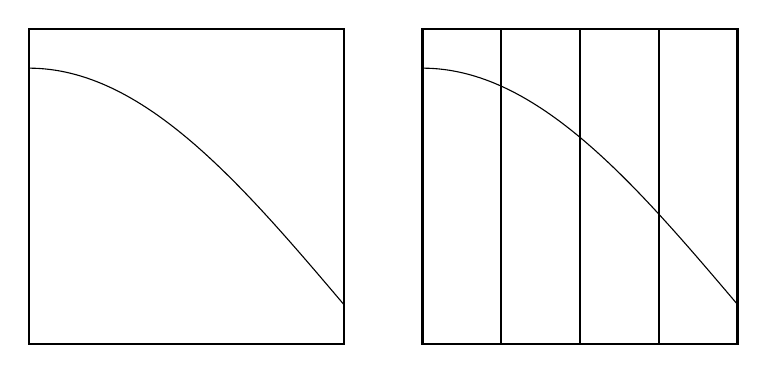
\begin{tikzpicture}
	\draw[thick] (0cm, 0cm) rectangle (4cm, 4cm);
	\foreach \x in {5cm, 6cm, 7cm, 8cm}
		\draw[thick] (\x, 0cm) rectangle (\x + 1 cm, 4cm);
	\draw (0,3.5) cos (4,0.5);
	\draw (5,3.5) cos (9,0.5);
\end{tikzpicture}
\caption{Wavelength and cell size}
\label{Wavelength-Vs-Cell-Size}
\end{figure}
% Reference for double figure: http://www.johndcook.com/blog/2009/01/14/how-to-display-side-by-side-figurs-in-latex/
\begin{figure}[htb]
\centering
\mbox{\subfigure[Gaussian pulse of width 2]{\includegraphics[scale=0.375, trim=3.75cm 8.75cm 4.5cm 9.25cm, clip]{Figures/FigCh02_Pulsewidth2.pdf}}\quad\subfigure[Gaussian pulse of width 4]{\includegraphics[scale=0.375, trim=3.75cm 8.75cm 4.5cm 9.25cm, clip]{Figures/FigCh02_Pulsewidth4.pdf}}}\\
\mbox{\subfigure[Gaussian pulse of width 8]{\includegraphics[scale=0.375, trim=3.75cm 8.75cm 4.5cm 9.25cm, clip]{Figures/FigCh02_Pulsewidth8.pdf}}\quad\subfigure[Gaussian pulse of width 16]{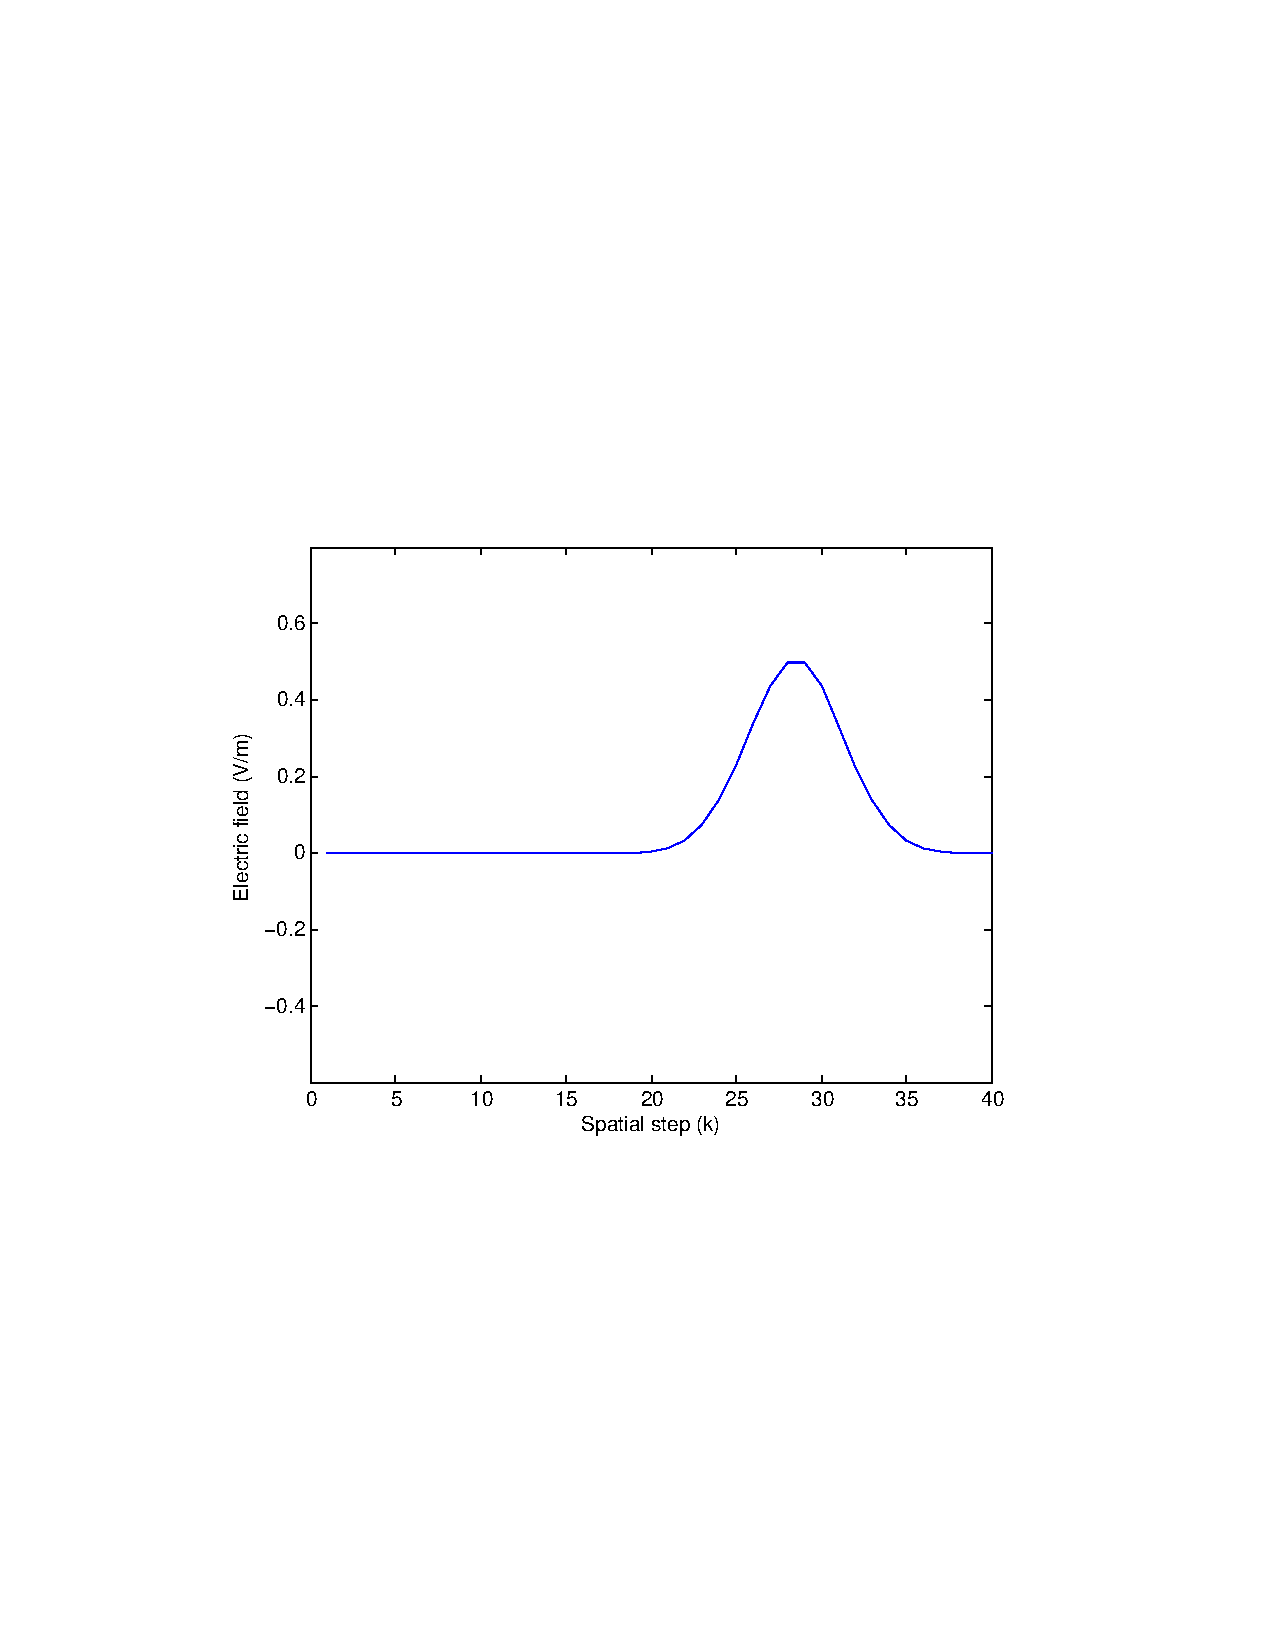
\includegraphics[scale=0.375, trim=3.75cm 8.75cm 4.5cm 9.25cm, clip]{Figures/FigCh02_Pulsewidth16.pdf}}}
\caption{Comparison of pulse width}
\label{Pulsewidth-comparison}
\end{figure}
Inaccuracies may also result from inappropriate selection of spatial or time steps. Figure~\ref{Unstable-FDTD} shows that FDTD\index{FDTD} quickly becomes unstable if $S_c$ becomes greater than unity. Further to this, FDTD\index{FDTD} is inherently dispersive\index{FDTD!dispersion} in nature and a pulse will spread as it travels over a period of time. While these inaccuracies cannot be completely eliminated, they can be reduced with proper selection of simulation parameters.
\section{Grid Termination and Boundary Conditions}
This section is a discussion on a number of grid termination conditions also known as boundary conditions. A graphical picture of different boundary conditions is given in figure~\ref{Boundary-Conditions}.
\subsection{Perfect Electric Conductor (PEC)\index{boundary condition!perfect electric conductor (PEC)}}
Where electric field nodes are located at the outermost boundary these can be set to zero to simulate a PEC boundary. A wave incident on PEC will be completely reflected with a 180 degree phase shift.
\subsection{Perfect Magnetic Conductor (PMC)\index{boundary condition!perfect magnetic conductor (PMC)}}
PMC is modelled by setting magnetic field nodes at edges set to zero. A PMC boundary will reflect incoming wave without any change in phase.
\subsection{Periodic Boundary Condition (PBC)\index{boundary condition!periodic (PBC)}}
In PBC incident waves will wrap around the and appear on the opposite edge. It is used to model the domain as a circular or continuous space. PBC boundary is implemented by incorporating the fields on edges in the FDTD update equations\index{FDTD!update equations}.
\subsection{Absorbing Boundary Condition (ABC)\index{boundary condition!absorbing (ABC)}}
An ABC will completely absorb incident fields without any reflection. This is useful for antenna radiation and scattering problems. There are a number of techniques for modelling ABCs, most popular being perfectly matched layer or PML\index{boundary condition!PML}.
\begin{figure}[H]
\centering
\mbox{\subfigure[Incident wave]{\includegraphics[scale=0.375, trim=3.75cm 8.75cm 4.5cm 9.25cm, clip]{Figures/FigCh02_Incident_Wave.pdf}}\quad\subfigure[Reflection from PMC]{\includegraphics[scale=0.375, trim=3.75cm 8.75cm 4.5cm 9.25cm, clip]{Figures/FigCh02_PMC_Reflected.pdf}}}
\mbox{\subfigure[Incident wave]{\includegraphics[scale=0.375, trim=3.75cm 8.75cm 4.5cm 9.25cm, clip]{Figures/FigCh02_Incident_Wave.pdf}}\quad\subfigure[Reflection from PEC]{\includegraphics[scale=0.375, trim=3.75cm 8.75cm 4.5cm 9.25cm, clip]{Figures/FigCh02_PEC_Reflected.pdf}}}
\mbox{\subfigure[Incident wave]{\includegraphics[scale=0.375, trim=3.75cm 8.75cm 4.5cm 9.25cm, clip]{Figures/FigCh02_Incident_Wave.pdf}}\quad\subfigure[Periodic boundary (PBC)]{\includegraphics[scale=0.375, trim=3.75cm 8.75cm 4.5cm 9.25cm, clip]{Figures/FigCh02_PBC.pdf}}}
\mbox{\subfigure[Incident wave]{\includegraphics[scale=0.375, trim=3.75cm 8.75cm 4.5cm 9.25cm, clip]{Figures/FigCh02_Incident_Wave.pdf}}\quad\subfigure[Absorbing boundary (ABC)]{\includegraphics[scale=0.375, trim=3.75cm 8.75cm 4.5cm 9.25cm, clip]{Figures/FigCh02_ABC.pdf}}}
\caption{Boundary Conditions: Incident wave is moving towards right.}
\label{Boundary-Conditions}
\end{figure}

% Drude model implementation of 1D and 2D DNG.
\chapter{FDTD Implementation of Metamaterials}
\section{Limitations of Standard FDTD Algorithm}
Standard FDTD\index{FDTD} algorithm cannot cater for negative values of permittivity or permeability. This is because of the Courant stability criterion\index{Courant stability criterion}. As soon as the permeability or permittivity becomes less than unity the algorithm will not remain stable. A metamaterial\index{metamaterial} object can be modelled as a dispersive substance using either the Lorentz\index{dispersive model!Lorentz} or Drude dispersive models\index{dispersive model!Drude}. These models can yield negative values of permittivity (or permeability) for certain frequency ranges~\cite{NumericalFDTD-Sibel}. Using these dispersive models, FDTD update equations\index{FDTD!update equations} are modified and permittivity and permeabilities are replaced with terms dependent on frequency of operation ($\omega$).
\section{Drude Dispersive Model}
In ideal conditions the permittivity (and permeability) of a material remain constant for any frequency and throughout the structure of that material. Speed of electromagnetic waves in such a medium remain constant if frequency changes. Additionally, there is no loss in energy as the waves pass through the medium.

In reality, such a material does not exist. Speed of EM waves varies with frequency of operation. Also, there is a loss associated with the material. A material is dispersive\index{dispersive material} if its permittivity or permeability is dependent on frequency~\cite[Ch. 10]{JBSchneiderUFDTD}.

This section follows the treatment of~\cite[Ch. 10, 289--290]{JBSchneiderUFDTD} for deriving permittivity relationship given by Drude model\index{dispersive model!Drude}. The Drude model is described by the following second order differential equation that relates the net force on charges moving under the influence of an electric field and facing an impeding force due to collisions\index{collision} with material.
\begin{equation}
\centering
M\dfrac{d^2 \textbf{x}}{dt^2} = Q \textbf{E}(t) - Mg\dfrac{d \textbf{x}}{dt}
\label{Drude-Model-Second-Order-DE}
\end{equation}
The left side of this equation gives mass times acceleration or the net force on charge. Here $M$ is the mass of charge, $Q$ the amount of charge, $\textbf{E}(t)$ is electric field that may vary with time and $g$ is the damping coefficient. Equation~\ref{Drude-Model-Second-Order-DE} can be converted to frequency domain using the relationships $\partial ^2/\partial t^2 \rightarrow (j\omega)^2$ and $\partial/\partial t \rightarrow j\omega$, obtaining
\begin{equation}
\centering
M(j\omega)^2\hat{\textbf{x}}(\omega)+Mg(j\omega)\hat{\textbf{x}}(\omega)=Q\hat{\textbf{E}}(\omega).
\label{Drude-Model-Second-Order-DE-Frequency-Domain}
\end{equation}
The polarization vector $\textbf{P}$ is given by
\begin{equation}
\centering
\hat{\textbf{P}}=NQ\hat{\textbf{x}}.
\label{Polarization}
\end{equation}
Here, $N$ is the number of dipoles per unit volume. By eliminating $\hat{\textbf{x}}$ from equations~\ref{Drude-Model-Second-Order-DE-Frequency-Domain} and~\ref{Polarization} and rearranging terms polarization can be expressed as
\begin{equation}
\centering
\hat{\textbf{P}}(\omega)=-\epsilon_0\dfrac{\frac{NQ^2}{M\epsilon_0}}{\omega^2-jg\omega}\hat{\textbf{E}}(\omega).
\label{Polarization-Frequency-Domain}
\end{equation}
By letting $\omega^2_p=NQ^2/M\epsilon_0$, the electric susceptibility is obtained as
\begin{equation}
\centering
\hat{\chi_e}(\omega)=-\dfrac{\omega^2_p}{\omega^2-jg\omega}.
\label{Electric-Susceptibility-Drude}
\end{equation}
The relative permittivity in Drude model\index{Drude model $\epsilon_r(\omega)$} is then
\begin{equation}
\centering
\hat{\epsilon_r}(\omega)=\epsilon_\infty-\dfrac{\omega^2_p}{\omega^2-jg\omega}.
\label{er-Drude}
\end{equation}
Setting $g=0$ and $\epsilon_\infty=1$, relative permittivity comes out to be negative for $\omega/\omega_p > 1$ (figure~\ref{DrudeModel_er}). Thus, Drude model can be effectively used to model metamaterials\index{metamaterial} with permittivity or permeability less than one by incorporating it into FDTD update equations.
\begin{figure}[H]
\centering
\includegraphics[scale=0.8, trim=4cm 8.5cm 4cm 8.5cm, clip]{Figures/FigCh03_DrudeModel_er.pdf}
\caption{$\epsilon_r$ plotted against $\omega/\omega_p$ for $\epsilon_\infty=1$ and $g=0$}
\label{DrudeModel_er}
\end{figure}
\section{FDTD Equations in 1D}
Here, the approach outlined in~\cite{Radial-Zhao} for derivation of FDTD auxiliary update equations is followed. Magnetic field $\textbf{H}$ and magnetic flux density $\textbf{B}$ are related by the constitutive parameter $\mu$, expressed as
\begin{equation}
\centering
\textbf{B} = \mu \textbf{H}.
\label{B-mu-H}
\end{equation}
Where, $\mu = \mu_0 \mu_r$. For a lossless, homogeneous, anisotropic and dispersion--less material, relative permeability or $\mu_r$ is a scalar constant. For dispersive material $\mu_r$ is a function of frequency. Similar to equation~\ref{er-Drude}, relative permeability for Drude model\index{Drude model $\mu_r(\omega)$} is given by
\begin{equation}
\begin{split}
\hat{\mu_r}(\omega)&=\mu_\infty-\dfrac{\omega^2_p}{\omega^2-jg\omega}\\
&=\dfrac{\mu_\infty(\omega^2-jg\omega)-\omega^2_p}{\omega^2-jg\omega}.
\end{split}
\label{ur-Drude}
\end{equation}
From equation~\ref{B-mu-H} and~\ref{ur-Drude},
\begin{equation}
\centering
\nonumber \textbf{B} \left( \dfrac{\omega^2-jg\omega}{\mu_\infty(\omega^2-jg\omega)-\omega^2_p} \right) =\textbf{H}
\label{B-muomega-H}
\end{equation}
and
\begin{equation}
\centering
\omega^2\textbf{B}-g(j\omega)\textbf{B} = \mu_\infty\omega^2\textbf{H}-\omega^2_p\textbf{H}-\mu_\infty g(j\omega)\textbf{H}.
\label{B-muomega-H-frequency-domain}
\end{equation}
Frequency domain quantities can be converted to time--domain using the relationships $j\omega \rightarrow \partial/\partial t$ and $\omega^2 \rightarrow - \partial^2/\partial t^2$. Moreover, fields multiplying with $\omega^2_p$ are averaged in time. Second--order difference scheme is used, both for single and double derivatives to keep all the terms in accordance with the second--order nature of whole expression. That would result in easier implementation. Assuming anisotropic nature of material, only $H_y$ and $B_y$ can be considered. Also, $\omega_{pm}$ and $\omega_{pe}$ are used for magnetic and electric field expressions instead of $\omega_p$, whereas, $\gamma_m$ and $\gamma_e$ are used for magnetic and electric collision frequencies\index{collision!frequency ($\gamma$)}, respectively.
\begin{equation}
\begin{split}
\left(\dfrac{B^{n+1}_y-2B^n_y+B^{n-1}_y}{(\Delta t)^2}\right)&+\gamma_m\left(\dfrac{B^{n+1}_y-B^{n-1}_y}{2\Delta t}\right) =\\
&\mu_0\mu_\infty\left(\dfrac{H^{n+1}_y-2H^n_y+H^{n-1}_y}{(\Delta t)^2}\right)\\
&+\mu_0\omega^2_{pm}\left(\dfrac{H^{n+1}_y+2H^n_y+H^{n-1}_y}{4}\right)\\
&+\mu_0\mu_\infty \gamma_m\left(\dfrac{H^{n+1}_y-H^{n-1}_y}{2\Delta t}\right).
\end{split}
\label{2nd-order-B-H}
\end{equation}
By separating $H^{n+1}_y$, the final form of equation is
\begin{eqnarray}
\nonumber H^{n+1}_y &=& a_m\left(B^{n+1}_y-2B^n_y+B^{n-1}_y\right)+b_m\left(B^{n+1}_y-B^{n-1}_y\right)\\
&&+c_m\left(2H^n_y-H^{n-1}_y\right)+d_m\left(2H^n_y+H^{n-1}_y\right)+e_m H^{n-1}_y.
\label{2nd-order-B-H-final-form}
\end{eqnarray}
Where,
\begin{eqnarray}
\nonumber & a_m=\dfrac{4}{4\mu_0\mu_\infty+\mu_0\omega^2_{pm}\left(\Delta t\right)^2+\mu_0\mu_\infty \gamma_m \left(2\Delta t\right)},\\
\nonumber & b_m=\dfrac{\gamma_m\left(2\Delta t\right)}{4\mu_0\mu_\infty+\mu_0\omega^2_{pm}\left(\Delta t\right)^2+\mu_0\mu_\infty \gamma_m \left(2\Delta t\right)},\\
\nonumber & c_m=\dfrac{4\mu_0\mu_\infty}{4\mu_0\mu_\infty+\mu_0\omega^2_{pm}\left(\Delta t\right)^2+\mu_0\mu_\infty \gamma_m \left(2\Delta t\right)},\\
\nonumber & d_m=\dfrac{-\mu_0\omega^2_{pm}\left(\Delta t\right)^2}{4\mu_0\mu_\infty+\mu_0\omega^2_{pm}\left(\Delta t\right)^2+\mu_0\mu_\infty \gamma_m \left(2\Delta t\right)},\\
\nonumber & e_m=\dfrac{\mu_0\mu_\infty \gamma_m\left(2\Delta t\right)}{4\mu_0\mu_\infty+\mu_0\omega^2_{pm}\left(\Delta t\right)^2+\mu_0\mu_\infty \gamma_m \left(2\Delta t\right)}.
\label{1D-Drude-H-scalars}
\end{eqnarray}
A similar derivation can be carried out to obtain the auxiliary update equation\index{FDTD!auxiliary update equation} for electric field given by
\begin{eqnarray}
\nonumber E^{n+1}_x &=& a_e\left(D^{n+1}_x-2D^n_x+D^{n-1}_x\right)+b_e\left(D^{n+1}_x-D^{n-1}_x\right)\\
&&+c_e\left(2E^n_x-E^{n-1}_x\right)+d_e\left(2E^n_x+E^{n-1}_x\right)+e_e E^{n-1}_x.
\label{2nd-order-D-E-final-form}
\end{eqnarray}
Where
\begin{eqnarray}
\nonumber & a_e=\dfrac{4}{4\epsilon_0\epsilon_\infty+\epsilon_0\omega^2_{pe}\left(\Delta t\right)^2+\epsilon_0\epsilon_\infty \gamma_e \left(2\Delta t\right)},\\
\nonumber & b_e=\dfrac{\gamma_e\left(2\Delta t\right)}{4\epsilon_0\epsilon_\infty+\epsilon_0\omega^2_{pe}\left(\Delta t\right)^2+\epsilon_0\epsilon_\infty \gamma_e \left(2\Delta t\right)},\\
\nonumber & c_e=\dfrac{4\epsilon_0\epsilon_\infty}{4\epsilon_0\epsilon_\infty+\epsilon_0\omega^2_{pe}\left(\Delta t\right)^2+\epsilon_0\epsilon_\infty \gamma_e \left(2\Delta t\right)},\\
\nonumber & d_e=\dfrac{-\epsilon_0\omega^2_{pe}\left(\Delta t\right)^2}{4\epsilon_0\epsilon_\infty+\epsilon_0\omega^2_{pe}\left(\Delta t\right)^2+\epsilon_0\epsilon_\infty \gamma_e \left(2\Delta t\right)},\\
\nonumber & e_e=\dfrac{\epsilon_0\epsilon_\infty \gamma_e\left(2\Delta t\right)}{4\epsilon_0\epsilon_\infty+\epsilon_0\omega^2_{pe}\left(\Delta t\right)^2+\epsilon_0\epsilon_\infty \gamma_e \left(2\Delta t\right)}.
\label{1D-Drude-E-scalars}
\end{eqnarray}
For a wave propagating in $z$ direction, FDTD update equations\index{FDTD!update equations} are
\begin{equation}
B^{n+1}_y(k)=B^n_y(k)+\dfrac{\Delta t}{\Delta z}\left(E^n_x(k)-E^n_x(k+1)\right)
\label{1D-B-Update-Equation}
\end{equation}
and
\begin{equation}
D^{n+1}_x(k)=D^n_x(k)+\dfrac{\Delta t}{\Delta z}\left(H^{n+1}_y(k-1)-H^{n+1}_y(k)\right).
\label{1D-D-Update-Equation}
\end{equation}
Equations \ref{1D-B-Update-Equation} and \ref{1D-D-Update-Equation} drive the FDTD algorithm which give future values of $By$ and $Dx$ from past fields. Equations \ref{2nd-order-B-H-final-form} and \ref{2nd-order-D-E-final-form} are auxiliary equations which give future fields $H_y$ and $E_x$ at $n+1$.
\section{Simulation of 1D DNG Slab}
\subsection{Problem Specification}
An electromagnetic wave travelling in $z$ direction is incident on a slab with negative values of permittivity and permeability (DNG)\index{DNG} at the frequency of operation \cite{DNG-Ehud-Ziol}. Sinusoidal wave\index{source!sinusoidal}, Gaussian pulse\index{source!Gaussian pulse} and Ricker wavelet\index{source!Ricker wavelet} are used as sources. Transmission\index{coefficient!transmission ($\tau$)} and reflection\index{coefficient!reflection ($\Gamma$)} coefficients are calculated at the air--slab interface. Refractive index of slab\index{refractive index ($n$)} for a range of frequencies is also computed. By varying parameters, the simulation can be scaled to any desired frequency or wavelength. Matlab\index{Matlab} code of this simulation is given in appendix \ref{App:1DFDTDDNGMatlab}.
\subsection{Implementation Details}
There are three main phases in the implementation:
\begin{enumerate}
\item Initialisation
\item Simulation
\item Post-processing
\end{enumerate}
Figure \ref{1D-DNG-Algorithm} depicts the flow of program.
\subsection{Initialisation}
In this phase, simulation parameters are specified. Simulation parameters are total number of spatial steps, time steps, wavelength and frequency of operation etc. Field arrays are then allocated and initialised. Any additional fields that are required for post--processing\index{post--processing} are also initialised. Arrays containing $\gamma_m$, $\gamma_e$, $\omega^2_{pm}$ and $\omega^2_{pe}$ must be initialised with values specified for each location in the domain.
\subsection{Simulation}
A dry run\index{dry run} must be carried out without any obstacle if reflection coefficient is to be calculated in order to record the incident field where obstacle is to be placed. The actual simulation consists of five steps:
\begin{enumerate}
\item Compute future value of $B_y$ from past values of $B_y$ and $E_x$ (equation \ref{1D-B-Update-Equation}).
\item Compute future value of $H_y$ from $B_y$ calculated in step 1 (equation \ref{2nd-order-B-H-final-form}).
\item Compute future value of $D_x$ from past value of $D_x$ and $H_y$ in step 2 (equation \ref{1D-D-Update-Equation}).
\item Compute future value of $E_x$ from $D_x$ calculated in step 3 (equation \ref{2nd-order-D-E-final-form}).
\item Update additive source at specified source location for current time step.
\end{enumerate}
Electric field snapshots are saved at specified intervals during simulation and played--back as a movie after simulation ends. 
\subsection{Post--processing}
After the simulation ends, reflection and transmission coefficients are calculated at the air--slab interface. Refractive index is calculated in the slab. A time--domain movie of the simulation is played that shows incident wave passing through the slab and undergoing dispersion.
\begin{figure}[htbp]
\centering
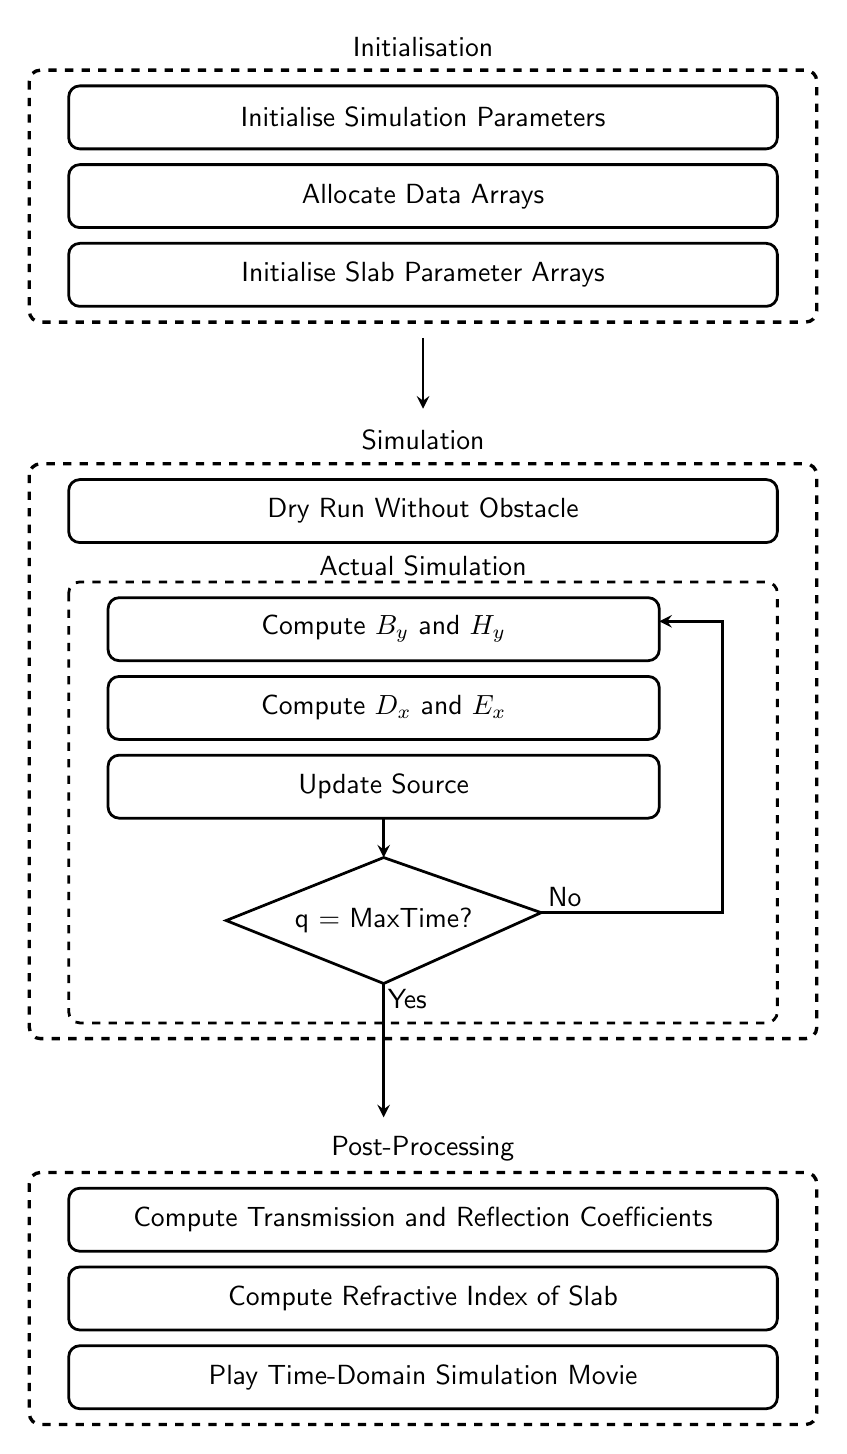
\begin{tikzpicture}
	% Initialisation.
	\draw (5cm,0.1cm) node {\textsf{Initialisation}};
	% Large dashed rectangle.
	\draw[line width=1.2pt, rounded corners, dashed] (0cm,-0.2cm) rectangle (10cm,-3.4cm);
	% Simulation parameters.
	\draw[line width=1pt, rounded corners] (0.5cm,-0.4cm) rectangle (9.5cm,-1.2cm);
	\draw (5cm,-0.8cm) node {\textsf{Initialise Simulation Parameters}};
	% Allocate data arrays.
	\draw[line width=1pt, rounded corners] (0.5cm,-1.4cm) rectangle (9.5cm,-2.2cm);
	\draw (5cm,-1.8cm) node {\textsf{Allocate Data Arrays}};
	% Initialise slab parameter arrays.
	\draw[line width=1pt, rounded corners] (0.5cm,-2.4cm) rectangle (9.5cm,-3.2cm);
	\draw (5cm,-2.8cm) node {\textsf{Initialise Slab Parameter Arrays}};
	\draw[line width=1pt, ->, >=stealth] (5cm,-3.6cm) -- (5cm,-4.5cm);

	% Simulation.
	\draw (5cm,-4.9cm) node {\textsf{Simulation}};
	% Large dashed rectangle.
	\draw[line width=1.2pt, rounded corners, dashed] (0cm,-5.2cm) rectangle (10cm,-12.5cm);
	% Dry run without obstacle.
	\draw[line width=1pt, rounded corners] (0.5cm,-5.4cm) rectangle (9.5cm,-6.2cm);
	\draw (5cm,-5.8cm) node {\textsf{Dry Run Without Obstacle}};
	% Actual Simulation.
	\draw[line width=1pt, rounded corners, dashed] (0.5cm,-6.7cm) rectangle (9.5cm,-12.3cm);
	\draw (5cm,-6.5cm) node {\textsf{Actual Simulation}};
	% Compute H fields.
	\draw[line width=1pt, rounded corners] (1.0cm,-6.9cm) rectangle (8.0cm,-7.7cm);
	\draw (4.5cm,-7.3cm) node {\textsf{Compute $B_y$ and $H_y$}};
	% Compute E fields.
	\draw[line width=1pt, rounded corners] (1.0cm,-7.9cm) rectangle (8.0cm,-8.7cm);
	\draw (4.5cm,-8.3cm) node {\textsf{Compute $D_x$ and $E_x$}};
	% Apply source.
	\draw[line width=1pt, rounded corners] (1.0cm,-8.9cm) rectangle (8.0cm,-9.7cm);
	\draw (4.5cm,-9.3cm) node {\textsf{Update Source}};
	\draw[line width=1pt, ->, >=stealth] (4.5cm,-9.7cm) -- (4.5cm,-10.2cm);
	% Diamond.
	\draw[line width=1pt] (4.5cm,-10.2cm) -- (2.5cm,-11cm) -- (4.5cm,-11.8cm) -- (6.5cm,-10.9cm) -- cycle;
	\draw (4.5cm,-11cm) node {\textsf{q = MaxTime?}};
	% No?
	\draw[line width=1pt, ->, >=stealth] (6.5cm,-10.9cm) -- (8.8cm,-10.9cm) -- (8.8cm,-7.2cm) -- (8.0cm,-7.2cm);
	\draw (6.8cm,-10.7cm) node {\textsf{No}};
	% Yes?
	\draw[line width=1pt, ->, >=stealth] (4.5cm,-11.8cm) -- (4.5cm,-12.7cm) -- (4.5cm,-12.7cm) -- (4.5cm,-13.5cm);
	\draw (4.8cm,-12.0cm) node {\textsf{Yes}};

	% Post-processing.
	\draw (5cm,-13.9cm) node {\textsf{Post-Processing}};
	% Large dashed rectangle.
	\draw[line width=1.2pt, rounded corners, dashed] (0cm,-14.2cm) rectangle (10cm,-17.4cm);
	% Transmission/Reflection coefficient calculations.
	\draw[line width=1pt, rounded corners] (0.5cm,-14.4cm) rectangle (9.5cm,-15.2cm);
	\draw (5cm,-14.8cm) node {\textsf{Compute Transmission and Reflection Coefficients}};
	% Refractive index calculations.
	\draw[line width=1pt, rounded corners] (0.5cm,-15.4cm) rectangle (9.5cm,-16.2cm);
	\draw (5cm,-15.8cm) node {\textsf{Compute Refractive Index of Slab}};
	% Simulation movie.
	\draw[line width=1pt, rounded corners] (0.5cm,-16.4cm) rectangle (9.5cm,-17.2cm);
	\draw (5cm,-16.8cm) node {\textsf{Play Time-Domain Simulation Movie}};
\end{tikzpicture}
\caption{Simulation algorithm}
\label{1D-DNG-Algorithm}
\end{figure}
\section{Simulation Results}
The simulation is run for both lossless and lossy cases with sinusoidal\index{source!sinusoidal}, Gaussian\index{source!Gaussian pulse} and Ricker\index{source!Ricker wavelet} wavelet sources. The slab parameters are set such that at frequency of operation, $f_0$, the permittivity and permeability of slab are both negative and result in a refractive index $n=-1$.
\subsection{Simulation Parameters}
The number of spatial steps is set as $4096$ and simulation is run for $4\times 4096$ time steps. The slab is located between steps $1365$ and $2731$. $\Delta z$ or spatial step is set as $3$ mm and time step, $\Delta t$, is set as $50$ ps. Frequency of operation is $f_0=0.1953125$ GHz and Courant number\index{Courant number ($S_c$)} for this configuration comes out to be $S_c=0.5$. In order to obtain relative permittivity and permeability of $-1$ at required $f_0$, plasma frequencies are set as $\omega^2_{pm}=\omega^2_{pe}=2\times(2\pi f_0)^2$ with $\epsilon_\infty=\mu_\infty=1$. First order absorbing boundary condition (ABC) are applied on fields at end points.
\subsection{Incident and Transmitted Fields}
Simulation with Gaussian pulse\index{source!Gaussian pulse} reveals that low frequency components are reflected at the interface which is confirmed from the transmission and reflection coefficients obtained for the air--slab interface. At $f_0$, the transmission coefficient is $1$ and there are no reflections when a sinusoidal source\index{source!sinusoidal} with $f_0$ is incident on the slab. Under steady--state conditions, transmitted wave inside the slab has negative phase velocity while energy is propagating in $+\hat{z}$ direction as expected.
\subsection{Refractive Index}
Following \cite{DNG-Ehud-Ziol}, the refractive index\index{refractive index ($n$)} was calculated from
\begin{equation}
n_{FDTD} = \dfrac{1}{jk_0(z_1-z_2)}log\left|\dfrac{E_x(\omega,z_2)}{E_x(\omega,z_1)}\right|.
\label{Refractive-Index-FDTD}
\end{equation}
Where, $k_0$ was the wave number\index{wave number ($k_0$)} set as $\omega_0/c$ and the fields were recorded at locations $z_1=1415\Delta z$ and $z_2=1424\Delta z$. For both, Gaussian\index{source!Gaussian pulse} pulse and Ricker\index{source!Ricker wavelet} wavelet, $Re(n)$ was $-1$ at $f_0$ while $Im(n)$ was sufficiently close to $0$.
\begin{figure}[H]
\centering
\includegraphics[scale=0.8, trim=3.5cm 8.7cm 4.5cm 8.85cm, clip]{Figures/FigCh03_IncidentFieldGaussian.pdf}
\caption{Gaussian pulse}
\label{1DDNG-IncidentField-Gaussian}
\end{figure}
\begin{figure}[H]
\centering
\includegraphics[scale=0.8, trim=3.5cm 8.7cm 4.5cm 8.85cm, clip]{Figures/FigCh03_IncidentFieldRicker.pdf}
\caption{Ricker wavelet}
\label{1DDNG-IncidentField-Ricker}
\end{figure}
\begin{figure}[H]
\centering
\includegraphics[scale=0.8, trim=3.5cm 8.7cm 4.5cm 8.85cm, clip]{Figures/FigCh03_IncidentFieldSinusoidal.pdf}
\caption{Sinusoidal wave}
\label{1DDNG-IncidentField-Sinusoidal}
\end{figure}
\begin{figure}[H]
\centering
\includegraphics[scale=0.8, trim=3.5cm 8.7cm 4.5cm 8.85cm, clip]{Figures/FigCh03_TransmissionReflectionCoefficient.pdf}
\caption{Transmission and reflection coefficients}
\label{1DDNG-Transmission-Reflection-Coefficient}
\end{figure}
\begin{figure}[H]
\centering
\includegraphics[scale=0.8, trim=3.5cm 8.7cm 4.5cm 8.85cm, clip]{Figures/FigCh03_TransmittedField.pdf}
\caption{Transmitted Gaussian pulse}
\label{1DDNG-Transmitted-Gaussian-Pulse}
\end{figure}
\begin{figure}[H]
\centering
\includegraphics[scale=0.8, trim=3.5cm 8.7cm 4.5cm 8.85cm, clip]{Figures/FigCh03_TransmittedFieldBeyondSlab.pdf}
\caption{Transmitted Gaussian pulse beyond slab}
\label{1DDNG-Transmitted-Gaussian-Pulse-Beyond-Slab}
\end{figure}
\begin{figure}[H]
\centering
\subfigure{\includegraphics[scale=0.8, trim=3.5cm 8.7cm 4.5cm 8.85cm, clip]{Figures/FigCh03_RefractiveIndex.pdf}}
\subfigure{\includegraphics[scale=0.8, trim=3.5cm 8.7cm 4.5cm 8.85cm, clip]{Figures/FigCh03_RefractiveIndexZoomed.pdf}}
\caption{Refractive index}
\label{1DDNG-Refractive-Index}
\end{figure}
\begin{figure}[H]
\centering
\includegraphics[scale=0.78, trim=3.5cm 8.7cm 4.5cm 8.75cm, clip]{Figures/FigCh03_1DDNGSteadyStateLossless.pdf}
\caption{Steady-state under lossless conditions}
\label{1DDNG-SteadyState-Lossless}
\end{figure}
\begin{figure}[H]
\centering
\includegraphics[scale=0.78, trim=3.5cm 8.7cm 4.5cm 8.75cm, clip]{Figures/FigCh03_1DDNGSteadyStateLossy.pdf}
\caption{Steady-state under lossy conditions}
\label{1DDNG-SteadyState-Lossy}
\end{figure}
\section{Simulation of 2D DNG Slab}
\subsection{Update Equations}
The most common 2D configurations are $TE^z$\index{polarisation!$TE^z$} or $TM^z$\index{polarisation!$TM^z$} polarisation where the problem space is confined to $xy$--plane. In $TE^z$, electric field components are transverse to $z$--axis and vice versa. For 2D simulation of DNG slab, $TM^z$ polarisation is assumed. The field components of interest would be $E_z$, $H_x$ and $H_y$. From equations \ref{Faraday's Law} and \ref{Ampere's Law},
\begin{equation}
\nabla \times \textbf{E} = -\dfrac{\partial \textbf{B}}{\partial t} = \left| \begin{array}{ccc} \hat{x} & \hat{y} & \hat{z} \\ \frac{\partial}{\partial x} & \frac{\partial}{\partial y} & \frac{\partial}{\partial z} \\ 0 & 0 & E_z \end{array} \right| = \dfrac{\partial E_z}{\partial y} \hat{x} - \dfrac{\partial E_z}{\partial x} \hat{y}
\label{eq:Faraday'sLawExpansionTMz}
\end{equation}
and
\begin{equation}
\nabla \times \textbf{H} = \dfrac{\partial \textbf{D}}{\partial t} = \left| \begin{array}{ccc} \hat{x} & \hat{y} & \hat{z} \\ \frac{\partial}{\partial x} & \frac{\partial}{\partial y} & \frac{\partial}{\partial z} \\ H_x & H_y & 0 \end{array} \right| = \dfrac{\partial H_y}{\partial x} \hat{z} - \dfrac{\partial H_x}{\partial y} \hat{z}.
\label{eq:Ampere'sLawExpansionTMz}
\end{equation}
The field components are given by scalar equations
\begin{equation}
\dfrac{\partial D_z}{\partial t} = \dfrac{\partial H_y}{\partial x} - \dfrac{\partial H_x}{\partial y},
\label{eq:partialofDzbyt}
\end{equation}
\begin{equation}
\dfrac{\partial B_x}{\partial t} = -\dfrac{\partial E_z}{\partial y}
\label{eq:partialofBxbyt}
\end{equation}
and
\begin{equation}
\dfrac{\partial B_y}{\partial t} = \dfrac{\partial E_z}{\partial x}.
\label{eq:partialofBybyt}
\end{equation}
FDTD update equations are obtained by discretising equations\index{FDTD!update equations} \ref{eq:partialofDzbyt}, \ref{eq:partialofBxbyt} and \ref{eq:partialofBybyt}, given by
\begin{equation}
\begin{split}
D^{n+1}_z \left[i,j\right]=D^{n}_z \left[i,j\right]+\dfrac{\Delta t}{\Delta}&\left(H^{n+\frac{1}{2}}_y\left[i+\frac{1}{2},j\right]-H^{n+\frac{1}{2}}_y \left[i-\frac{1}{2},j\right]\right.\\
&\left.-H^{n+\frac{1}{2}}_x \left[i,j+\frac{1}{2}\right]+H^{n+\frac{1}{2}}_x \left[i,j-\frac{1}{2}\right]\right),
\end{split}
\label{eq:Dz-2D-FDTD-TMz}
\end{equation}
\begin{equation}
B^{n+\frac{1}{2}}_x \left[i,j+\frac{1}{2}\right]=B^{n-\frac{1}{2}}_x \left[i,j+\frac{1}{2}\right] + \dfrac{\Delta t}{\Delta} \left(-E^{n}_z \left[i,j+1\right] + E^{n}_z \left[i,j\right] \right)
\label{eq:Bx-2D-FDTD-TMz}
\end{equation}
and
\begin{equation}
B^{n+\frac{1}{2}}_y \left[i+\frac{1}{2},j\right]=B^{n-\frac{1}{2}}_y \left[i+\frac{1}{2},j\right] + \dfrac{\Delta t}{\Delta} \left( E^{n}_z \left[i+1,j\right] - E^{n}_z \left[i,j\right] \right).
\label{eq:By-2D-FDTD-TMz}
\end{equation}
It is important to note here that DNG slab medium is assumed anisotropic. The auxiliary update equations\index{FDTD!auxiliary update equation} (\ref{2nd-order-B-H-final-form} and \ref{2nd-order-D-E-final-form}) to obtain electric and magnetic fields, $E_v$ and $H_v$ ($v\in x,y,z$), from corresponding flux densities, $D_v$ and $B_v$, remain unchanged.
\subsection{Simulation Geometry}
The DNG slab interface is perpendicular to incident plane wave\index{plane wave} propagating in $+y$ direction. Periodic boundary conditions (PBC)\index{boundary condition!periodic (PBC)} are applied at $x=0$ and $x=x_{max}$. In $y$ direction the grid is terminated at both ends by perfectly matched layer (PML)\index{boundary condition!PML} to absorb any incoming waves. The solution geometry is depicted in figure \ref{fig:2D-DNG-Geometry}. The arrangement of field nodes is shown in figure \ref{fig:2D-DNG-Field-Nodes}.  Magnetic field components are updated first and then used to update electric field.

The solution space is bounded in $y$ direction at both ends by $H_x$ which acts as the boundary for PML. $H_x$ at these end points is set to 0 so that any out--going fields are reflected back into PML. Essentially, the $j$ size of $H_x$ arrays is one greater than $H_y$ and $E_z$ arrays. This arrangement results in following update equations that can be directly programmed, taking into account discrete indices for field storage.
\begin{equation}
\begin{split}
D^{n+1}_z \left[i,j\right]=D^{n}_z \left[i,j\right]+\dfrac{\Delta t}{\Delta}&\left(H^{n+1}_y\left[i,j\right]-H^{n+1}_y \left[i-1,j\right]\right.\\
&\left.-H^{n+1}_x \left[i,j+1\right]+H^{n+1}_x \left[i,j\right]\right).
\end{split}
\label{eq:Dz-2D-FDTD-TMz-Corrected}
\end{equation}
\begin{equation}
B^{n+1}_x \left[i,j\right]=B^n_x \left[i,j\right] + \dfrac{\Delta t}{\Delta} \left(-E^{n}_z \left[i,j\right] + E^{n}_z \left[i,j-1\right] \right).
\label{eq:Bx-2D-FDTD-TMz-Corrected}
\end{equation}
\begin{equation}
B^{n+1}_y \left[i,j\right]=B^n_y \left[i,j\right] + \dfrac{\Delta t}{\Delta} \left( E^{n}_z \left[i+1,j\right] - E^{n}_z \left[i,j\right] \right).
\label{eq:By-2D-FDTD-TMz-Corrected}
\end{equation}
\subsection{Simulation Parameters and Results}
The solution space is 512 cells in both $x$ and $y$ directions without taking into account the width of PML, which is 50 cells wide. The plane wave source is located 10 cells from the lower PML layer. The spatial and temporal steps are set as $\Delta x=\Delta y=\Delta=3$ mm and $\Delta t=50$ ps, respectively; with a Courant number of 0.5\index{Courant number ($S_c$)}. Frequency of operation is $f_0=1.5625$ GHz. The DNG slab parameters are same as in the case of 1D DNG simulation.

Figure \ref{fig:2DDNG-Refractive-Index} shows the refractive index\index{refractive index ($n$)} obtained for a range of frequencies with a Gaussian pulse excitation. Again, real part of refractive index at $f_0$ is close to -1, whereas, imaginary part is close to 0. Figure \ref{fig:2DDNG-SteadyState-Lossy} shows sinusoidal steady--state\index{steady--state} under lossy conditions where the source is located towards left and incident plane wave is moving rightwards. Under lossless conditions the slab can act as a perfect lens\index{perfect lens} (figure \ref{fig:2DDNG-Slab-lens}).
\begin{figure}[H]
\centering
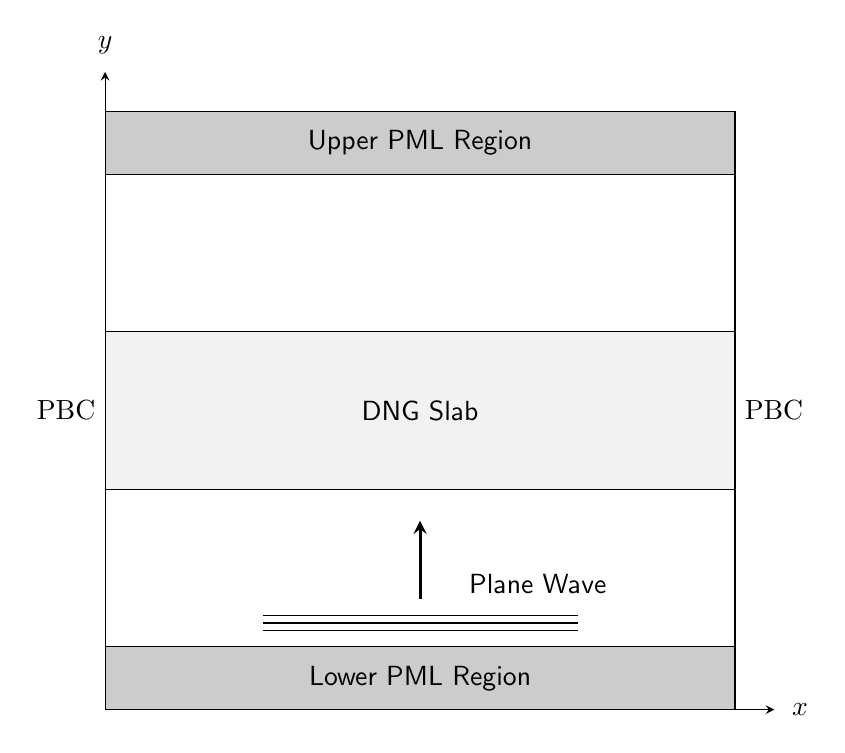
\begin{tikzpicture}
	\newcommand{\LeftX}{0cm}
	\newcommand{\MidX}{4cm}
	\newcommand{\RightX}{8cm}
	\newcommand{\PMLw}{0.8cm}
	\newcommand{\DomainY}{6.0cm}
	\newcommand{\SlabStartY}{2.0cm+\PMLw}
	\newcommand{\SlabEndY}{4.0cm+\PMLw}
	% x-axis.
	\draw[->, >=stealth] (\LeftX,0cm) -- (\RightX+0.5cm,0cm);
	\coordinate [label=right:$x$] (x-axis) at (\RightX+0.6cm,0cm);
	% y-axis.
	\draw[->, >=stealth] (\LeftX,0cm) -- (\LeftX,2*\PMLw+\DomainY+0.5cm);
	\coordinate [label=above:$y$] (y-axis) at (\LeftX,2*\PMLw+\DomainY+0.6cm);
	% PBCs.
	\coordinate [label=right:PBC] (PBCright) at (\RightX,\PMLw+3.0cm);
	\coordinate [label=left:PBC] (PBCleft) at (\LeftX,\PMLw+3.0cm);
	% Lower PML Region.
	\draw[fill=gray!40!white] (\LeftX,0cm) rectangle (\RightX,\PMLw);
	\coordinate [label=center:\textsf{Lower PML Region}] (LowerPML) at (\MidX,0.4cm);
	% Solution Region.
	\draw (\LeftX,\PMLw) rectangle (\RightX,\PMLw+\DomainY);
	% Upper PML Region.
	\draw[fill=gray!40!white] (\LeftX,\PMLw+\DomainY) rectangle (\RightX,2*\PMLw+\DomainY);
	\coordinate [label=center:\textsf{Upper PML Region}] (UpperPML) at (\MidX,\PMLw+\DomainY+0.4cm);
	% Slab.
	\draw[fill=gray!10!white] (\LeftX,\SlabStartY) rectangle (\RightX,\SlabEndY);
	\coordinate [label=center:\textsf{DNG Slab}] (DNGSlab) at (\MidX,\PMLw+3.0cm);
	% Plane wave.
	\draw (\LeftX+2.0cm,\PMLw+0.2cm) -- (\RightX-2.0cm, \PMLw+0.2cm);
	\draw (\LeftX+2.0cm,\PMLw+0.3cm) -- (\RightX-2.0cm, \PMLw+0.3cm);
	\draw (\LeftX+2.0cm,\PMLw+0.4cm) -- (\RightX-2.0cm, \PMLw+0.4cm);
	\draw[line width=1.1pt, ->, >=stealth] (\MidX,\PMLw+0.6cm) -- (\MidX,\PMLw+1.6cm);
	\coordinate [label=right:\textsf{Plane Wave}] (PlaneWave) at (\MidX+0.5cm,\PMLw+0.8cm);
\end{tikzpicture}
\caption{Simulation geometry}
\label{fig:2D-DNG-Geometry}
\end{figure}
\begin{figure}[H]
\centering
\begin{tikzpicture}
	\newcommand{\LeftX}{0cm}
	\newcommand{\RightX}{5cm}
	\newcommand{\LowY}{0cm}
	\newcommand{\HighY}{5.5cm}
	% x-axis.
	\draw[->, >=stealth] (\LeftX,\LowY) -- (\RightX,\LowY);
	\coordinate [label=right:$x$] (x-axis) at (\RightX+0.1cm,\LowY);
	% y-axis.
	\draw[->, >=stealth] (\LeftX,\LowY) -- (\LeftX,\HighY);
	\coordinate [label=above:$y$] (y-axis) at (\LeftX,\HighY+0.1cm);
	% Drawing vertical grid lines.
	\foreach \x in {1cm,2cm,3cm,4cm}
		\draw (\x,\LowY-0.1cm) -- (\x,\HighY-0.25cm); % Solid lines at +1 intervals.
	\foreach \x in {0.5cm,1.5cm,2.5cm,3.5cm,4.5cm}
		\draw[dashed] (\x,\LowY) -- (\x,\HighY-0.25cm); % Dashed lines at 1/2 intervals.
	% Drawing horizontal grid lines.
	\foreach \y in {1cm,2cm,3cm,4cm,5cm}
		\draw (\LeftX-0.1cm,\y) -- (\RightX-0.25cm,\y); % Solid lines at +1 intervals.
	\foreach \y in {0.5cm,1.5cm,2.5cm,3.5cm,4.5cm}
		\draw[dashed] (\LeftX,\y) -- (\RightX-0.25cm,\y); % Dashed lines at 1/2 intervals.
	% Drawing nodes.
	\foreach \x in {0cm,1cm,2cm,3cm,4cm}
		\foreach \y in {0.5cm,1.5cm,2.5cm,3.5cm,4.5cm}
			\filldraw (\x,\y) circle (0.08cm); % Ez nodes.
	\foreach \x in {0.5cm,1.5cm,2.5cm,3.5cm,4.5cm}
		\foreach \y in {0.5cm,1.5cm,2.5cm,3.5cm,4.5cm}
			\node[fill=black,regular polygon, regular polygon sides=4,inner sep=0.05cm] at (\x,\y) {}; % Hy nodes.
	\foreach \x in {0cm,1cm,2cm,3cm,4cm}
		\foreach \y in {0cm,1cm,2cm,3cm,4cm,5cm}
			\node[fill=black,regular polygon, regular polygon sides=3,inner sep=0.04cm] at (\x,\y) {}; % Hx nodes.
	% +1 Text for x-axis.
	\foreach \x/\t in {0cm/0,1cm/1,2cm/2,3cm/3,4cm/4}
		\coordinate [label=below:$\t$] (\t) at (\x,\LowY-0.2cm);
	% 1/2 Text for x-axis.
	\foreach \x/\t in {0.5cm/ ,1.5cm/1,2.5cm/2,3.5cm/3,4.5cm/4}
		\coordinate [label=below:{\tiny $\t\frac{1}{2}$}] (\t) at (\x,\LowY-0.2cm);
	% +1 Text for y-axis.
	\foreach \y/\t in {0cm/0,1cm/1,2cm/2,3cm/3,4cm/4,5cm/5}
		\coordinate [label=left:$\t$] (\t) at (\LeftX-0.2cm,\y);
	% 1/2 Text for y-axis.
	\foreach \y/\t in {0.5cm/ ,1.5cm/1,2.5cm/2,3.5cm/3,4.5cm/4}
		\coordinate [label=left:{\tiny $\t\frac{1}{2}$}] (\t) at (\LeftX-0.2cm,\y);
	% Legend
	\filldraw (\LeftX+0cm,\LowY-1cm) circle (0.08cm); % Ez.
	\coordinate [label=center:$E_z$] (EzLegend) at (\LeftX+0.4cm,\LowY-1cm);
	\node[fill=black,regular polygon, regular polygon sides=3,inner sep=0.04cm] at (\LeftX+1cm,\LowY-1cm) {}; % Hx.
	\coordinate [label=center:$H_x$] (HxLegend) at (\LeftX+1.4cm,\LowY-1cm);
	\node[fill=black,regular polygon, regular polygon sides=4,inner sep=0.05cm] at (\LeftX+2cm,\LowY-1cm) {}; % Hy.
	\coordinate [label=center:$H_y$] (HxLegend) at (\LeftX+2.4cm,\LowY-1cm);
\end{tikzpicture}
\caption{Arrangement of field nodes}
\label{fig:2D-DNG-Field-Nodes}
\end{figure}
\begin{figure}[H]
\centering
\subfigure{\includegraphics[scale=0.8, trim=3.5cm 8.7cm 4.5cm 8.85cm, clip]{Figures/FigCh03_2DDNGRefractiveIndex.pdf}}
\subfigure{\includegraphics[scale=0.8, trim=3.5cm 8.7cm 4.5cm 8.85cm, clip]{Figures/FigCh03_2DDNGRefractiveIndexZoomed.pdf}}
\caption{Refractive index of 2D DNG slab}
\label{fig:2DDNG-Refractive-Index}
\end{figure}
\begin{figure}[H]
\centering
\subfigure{\includegraphics[scale=0.5, trim=1.0cm 0.05cm 1.75cm 0cm, clip]{Figures/FigCh03_2DDNGSteadyStateLossy.png}}
\subfigure{\includegraphics[scale=0.5, trim=1.0cm 0.05cm 1.75cm 0cm, clip]{Figures/FigCh03_2DDNGSteadyStateLossyOverhead.png}}
\caption{Steady-state under lossy conditions for 2D DNG slab}
\label{fig:2DDNG-SteadyState-Lossy}
\end{figure}
\begin{figure}[H]
\centering
\subfigure{\includegraphics[scale=0.5, trim=1.0cm 0.05cm 1.75cm 0cm, clip]{Figures/FigCh03_2DDNGSlabLensSideView.png}}
\subfigure{\includegraphics[scale=0.5, trim=1.0cm 0.05cm 1.75cm 0cm, clip]{Figures/FigCh03_2DDNGSlabLens.png}}
\caption{DNG slab as lens: source is located towards left}
\label{fig:2DDNG-Slab-lens}
\end{figure}

% 1D and 2D DNG on C++ and GPU
\chapter{GPU Implementation of 1D and 2D DNG Slab}
\section{GPU Programming Model\index{GPU!programming model}}
\subsection{Evolution of GPUs\index{GPU!evolution}}
With the evolution of 3D graphics arose a need for faster computing means to handle real--time graphics processing. The graphics processing unit or GPU\index{GPU} was originally meant to act as a separate processor to handle graphics computations. The process of transforming a 3D scenario to a 2D image that can be displayed on a computer screen is known as \emph{rendering}\index{render}. Rendering involves determining the exact colour or shade of each pixel and geometry calculations. In the earliest GPUs these were referred to as pixel\index{shader!pixel} and vertex\index{shader!vertex} shading. The GPUs had discrete processing units known as pixel and vertex shaders that performed these calculations. As an example, the nVidia's\index{nVidia} GeForce 6200 GPU had four pixel shaders and three vertex shaders \cite{Ref:Geforce6-wiki}. Table \ref{Tab:Eary-GPU-Comparison} provides a comparison of some typical GPUs. The number of pixel shaders are significantly greater than vertex shaders due to unequal workload.
\begin{table}[H]
\begin{center}
\vspace{0.3cm}
	\begin{tabular}{lccc}
	\hline \hline
		\rule{0pt}{2.6ex} & \textbf{GeForce 6200} & \textbf{GeForce 6600} & \textbf{ATi x850}\\
		\hline
		Transistor Count \rule{0pt}{2.6ex} & 77 million & 222 million & 160 million\\
		Process & 0.11 $\mu$m & 0.11 $\mu$m & 0.13 $\mu$m low--k\\
		Pixel Shaders & 4 & 8 & 16\\
		Vertex Shaders & 3 & 3 & 6\\
	\hline \hline
	\end{tabular}
\end{center}
\caption{Comparison of some early GPUs}
\label{Tab:Eary-GPU-Comparison}
\end{table}
\subsection{Unified Shader Architecture\index{unified shader!architecture}}
GPUs\index{GPU} were already far ahead of contemporary CPUs\index{CPU} in terms of computation power when the first line of these new GPUs based on unified shader model\index{unified shader!architecture} arrived in 2005 \cite{Ref:Unified-Shader-Architecture-devmaster.net}. In the unified shader model\index{unified shader!model} shading units are not confined to just pixel or vertex calculations. They can operate on any \emph{shader instruction}\index{shader!instruction} \cite{Ref:Unified-Shader-Model-wiki}. Each shader is capable of doing same set of defined arithmetic calculations. It was possible to use GPU as a general-purpose computing device\index{GPU!general purpose (GPGPU)}.

Major GPU manufacturers, nVidia\index{nVidia} and AMD/ATi\index{AMD/ATi} provide application programming interface (API)\index{API} and software development kits (SDKs)\index{SDK} to program their GPUs. CUDA\index{CUDA} or compute unified device architecture is the API provided by nVidia to program their GPUs. Additionally, an open standard OpenCL\index{OpenCL} has evolved for GPU computing that has been adopted by both nVidia and AMD/ATi. AMD/ATi API is based on OpenCL standard.

To take advantage of GPU acceleration a problem must have either task--parallel or data--parallel nature.
\subsection{Task--Parallelism\index{parallelism!task}}
In task--parallelism computation consist of several independent tasks that run concurrently. These tasks may be completely unrelated but the end result is dependent on their outputs. Consider summation of a series, where we want to compute the value of $e^x$ from Taylor series. The mathematical expression is given by
\begin{equation}
e^x = 1+\dfrac{x^1}{1!}+\dfrac{x^2}{2!}+\dfrac{x^3}{3!}+\dfrac{x^4}{4!}+\dfrac{x^5}{5!}+\dfrac{x^6}{6!}+...+\dfrac{x^n}{n!}
\label{eq:ex-Taylor-Series}
\end{equation}

A single--threaded\index{threading!single} conventional implementation would have to calculate all the terms one--by--one and then sum up the result in the end. However, in a multi--threaded\index{threading!multi} implementation, each thread would calculate only one term. All the treads will perform their computation in parallel and the end result is then summed up. The computation--intensive task of calculating factorials and higher powers of $x$ is parallelised and results in significant reduction of computation time.
\subsection{Data--Parallelism\index{parallelism!data}}
In data--parallelism same operation is performed on individual elements of data. A simple example is that of scalar matrix multiplication. Consider an array of size $n$ being multiplied with a scalar constant $c$. The result of each multiplication can be calculated independently by assigning a separate thread for the task. This is illustrated in figure \ref{fig:Data-Parallelism} where input array is \texttt{A[]} and resultant array is \texttt{B[]}. Data--parallelism applies to any scenario where values in resultant data array only depends on values from input array. FDTD\index{FDTD!data--parallelism} is a good example of data--parallelism and a GPU implementation can take advantage of accelerated computing.
\begin{figure}[H]
\centering
\subfigure[Single--threaded implementation]{
\begin{tikzpicture}
	\newcommand{\Xdisp}{0cm}
	\newcommand{\Ydisp}{0cm}
	% e^x;
	\coordinate [label=center:$e^x\rightarrow$] (exequals) at (\Xdisp-0.75cm,\Ydisp+0.75cm);
	% Single-threaded flow chart.
	\draw (\Xdisp-0.25cm,\Ydisp+0.75cm) -- (\Xdisp+0.5cm,\Ydisp+0.75cm) -- (\Xdisp+0.5cm,\Ydisp);
	\draw (\Xdisp,\Ydisp) rectangle (\Xdisp+1.0cm,\Ydisp-1.0cm);
	\coordinate [label=center:$\dfrac{x^0}{0!}$] (Term0ST) at (\Xdisp+0.5cm,\Ydisp-0.5cm);

	\renewcommand{\Xdisp}{1.25cm}
	\renewcommand{\Ydisp}{-1.25cm}
	\draw (\Xdisp-0.25cm,\Ydisp+0.75cm) -- (\Xdisp+0.5cm,\Ydisp+0.75cm) -- (\Xdisp+0.5cm,\Ydisp);
	\draw (\Xdisp,\Ydisp) rectangle (\Xdisp+1.0cm,\Ydisp-1.0cm);
	\coordinate [label=center:$\dfrac{x^1}{1!}$] (Term1ST) at (\Xdisp+0.5cm,\Ydisp-0.5cm);
	\filldraw[fill=white] (\Xdisp+0.5cm,\Ydisp+0.75cm) circle (0.25cm);
	\coordinate [label=center:$+$] (plusTerm1ST) at (\Xdisp+0.5cm,\Ydisp+0.75cm);

	\renewcommand{\Xdisp}{2.5cm}
	\renewcommand{\Ydisp}{-2.5cm}
	\draw (\Xdisp-0.25cm,\Ydisp+0.75cm) -- (\Xdisp+0.5cm,\Ydisp+0.75cm) -- (\Xdisp+0.5cm,\Ydisp);
	\draw (\Xdisp,\Ydisp) rectangle (\Xdisp+1.0cm,\Ydisp-1.0cm);
	\coordinate [label=center:$\dfrac{x^2}{2!}$] (Term2ST) at (\Xdisp+0.5cm,\Ydisp-0.5cm);
	\filldraw[fill=white] (\Xdisp+0.5cm,\Ydisp+0.75cm) circle (0.25cm);
	\coordinate [label=center:$+$] (plusTerm2ST) at (\Xdisp+0.5cm,\Ydisp+0.75cm);

	\renewcommand{\Xdisp}{3.75cm}
	\renewcommand{\Ydisp}{-3.75cm}
	\draw (\Xdisp-0.25cm,\Ydisp+0.75cm) -- (\Xdisp+0.5cm,\Ydisp+0.75cm) -- (\Xdisp+0.5cm,\Ydisp);
	\draw (\Xdisp,\Ydisp) rectangle (\Xdisp+1.0cm,\Ydisp-1.0cm);
	\coordinate [label=center:$\dfrac{x^3}{3!}$] (Term3ST) at (\Xdisp+0.5cm,\Ydisp-0.5cm);
	\filldraw[fill=white] (\Xdisp+0.5cm,\Ydisp+0.75cm) circle (0.25cm);
	\coordinate [label=center:$+$] (plusTerm3ST) at (\Xdisp+0.5cm,\Ydisp+0.75cm);

	\renewcommand{\Xdisp}{5cm}
	\renewcommand{\Ydisp}{-5cm}
	\draw[dashed] (\Xdisp-0.25cm,\Ydisp+0.75cm) -- (\Xdisp+0.5cm,\Ydisp+0.75cm) -- (\Xdisp+0.5cm,\Ydisp);
	\draw (\Xdisp,\Ydisp) rectangle (\Xdisp+1.0cm,\Ydisp-1.0cm);
	\coordinate [label=center:$\dfrac{x^n}{n!}$] (TermnST) at (\Xdisp+0.5cm,\Ydisp-0.5cm);
	\filldraw[fill=white] (\Xdisp+0.5cm,\Ydisp+0.75cm) circle (0.25cm);
	\coordinate [label=center:$+$] (plusTermnST) at (\Xdisp+0.5cm,\Ydisp+0.75cm);
	% Result
	\coordinate [label=right:$\rightarrow$\textsf{Result}] (ResultST) at (\Xdisp+1.0cm,\Ydisp-0.5cm);
	% Thread.
	\draw[thick, rounded corners, ->, >=stealth] (-0.75cm,-0.5cm) -- (-0.9cm,-0.75cm) -- (-0.6cm,-1.25cm) -- (-0.9cm,-1.75cm) -- (-0.6cm,-2.25cm) -- (-0.9cm,-2.75cm) -- (-0.6cm,-3.25cm) -- (-0.9cm,-3.75cm) -- (-0.6cm,-4.25cm) -- (-0.9cm,-4.75cm) -- (-0.75cm,-5.0cm) -- (-0.75cm,-5.5cm);
\end{tikzpicture}}
\subfigure[Multi--threaded implementation]{
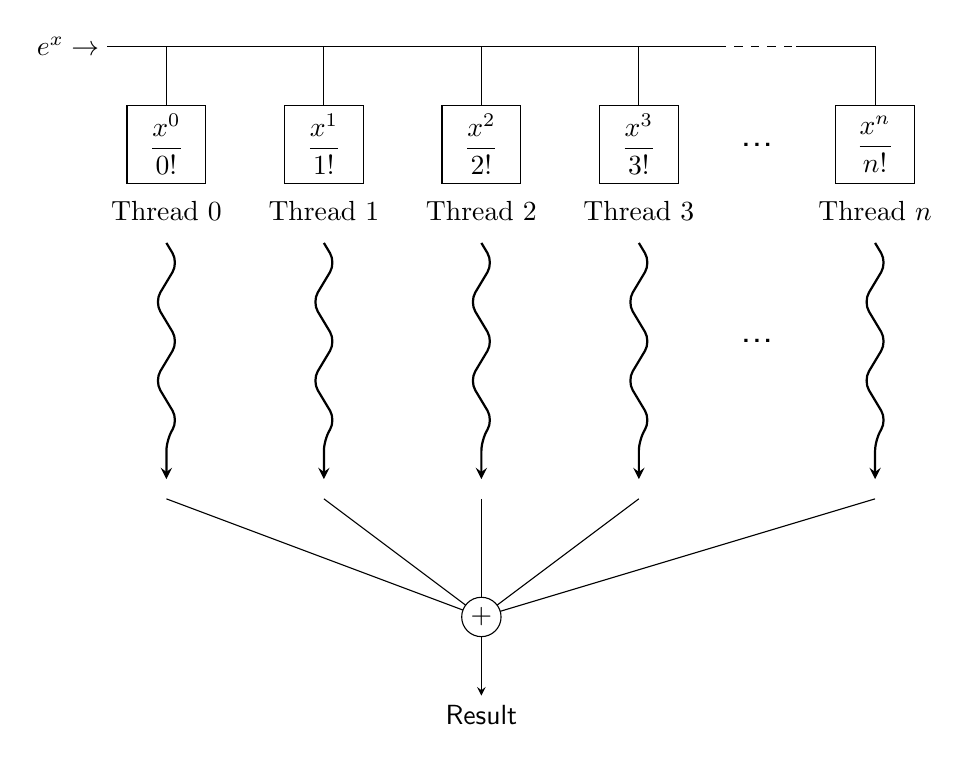
\begin{tikzpicture}
	\newcommand{\Xdisp}{0cm}
	\newcommand{\Ydisp}{0cm}
	% e^x;
	\coordinate [label=center:$e^x\rightarrow$] (exequals) at (\Xdisp-0.75cm,\Ydisp+0.75cm);
	% Single-threaded flow chart.
	\draw (-0.25cm,\Ydisp+0.75cm) -- (\Xdisp+0.5cm,\Ydisp+0.75cm) -- (\Xdisp+0.5cm,\Ydisp);
	\draw (\Xdisp,\Ydisp) rectangle (\Xdisp+1.0cm,\Ydisp-1.0cm);
	\coordinate [label=center:$\dfrac{x^0}{0!}$] (Term0MT) at (\Xdisp+0.5cm,\Ydisp-0.5cm);

	\renewcommand{\Xdisp}{2cm}
	\draw (-0.25cm,\Ydisp+0.75cm) -- (\Xdisp+0.5cm,\Ydisp+0.75cm) -- (\Xdisp+0.5cm,\Ydisp);
	\draw (\Xdisp,\Ydisp) rectangle (\Xdisp+1.0cm,\Ydisp-1.0cm);
	\coordinate [label=center:$\dfrac{x^1}{1!}$] (Term1MT) at (\Xdisp+0.5cm,\Ydisp-0.5cm);

	\renewcommand{\Xdisp}{4cm}
	\draw (-0.25cm,\Ydisp+0.75cm) -- (\Xdisp+0.5cm,\Ydisp+0.75cm) -- (\Xdisp+0.5cm,\Ydisp);
	\draw (\Xdisp,\Ydisp) rectangle (\Xdisp+1.0cm,\Ydisp-1.0cm);
	\coordinate [label=center:$\dfrac{x^2}{2!}$] (Term2MT) at (\Xdisp+0.5cm,\Ydisp-0.5cm);

	\renewcommand{\Xdisp}{6cm}
	\draw (-0.25cm,\Ydisp+0.75cm) -- (\Xdisp+0.5cm,\Ydisp+0.75cm) -- (\Xdisp+0.5cm,\Ydisp);
	\draw (\Xdisp,\Ydisp) rectangle (\Xdisp+1.0cm,\Ydisp-1.0cm);
	\coordinate [label=center:$\dfrac{x^3}{3!}$] (Term3MT) at (\Xdisp+0.5cm,\Ydisp-0.5cm);

	% Dots.
	\coordinate [label=center:\textsf{{\Large ...}}] (Dots1) at (8cm,\Ydisp-0.5cm);
	\coordinate [label=center:\textsf{{\Large ...}}] (Dots2) at (8cm,\Ydisp-3cm);

	\renewcommand{\Xdisp}{9cm}
	\draw (-0.25cm,\Ydisp+0.75cm) -- (\Xdisp-1.5cm,\Ydisp+0.75cm);
	\draw[dashed] (\Xdisp-1.5cm,\Ydisp+0.75cm) -- (\Xdisp-0.5cm,\Ydisp+0.75cm);
	\draw (\Xdisp-0.5cm,\Ydisp+0.75cm) -- (\Xdisp+0.5cm,\Ydisp+0.75cm) -- (\Xdisp+0.5cm,\Ydisp);
	\draw (\Xdisp,\Ydisp) rectangle (\Xdisp+1.0cm,\Ydisp-1.0cm);
	\coordinate [label=center:$\dfrac{x^n}{n!}$] (TermnMT) at (\Xdisp+0.5cm,\Ydisp-0.5cm);

	% Thread numbers.
	\foreach \x/\t in {0.5cm/0,2.5cm/1,4.5cm/2,6.5cm/3,9.5cm/n}
		\coordinate [label=below:Thread $\t$] (Thread\t) at (\x,-1.1cm);
	% Threads.
	\foreach \x in {0.5cm,2.5cm,4.5cm,6.5cm,9.5cm}
		\draw[thick, rounded corners, ->, >=stealth] (\x+0cm,-1.75cm) -- (\x+0.15cm,-2cm) -- (\x-0.15cm,-2.5cm) -- (\x+0.15cm,-3cm) -- (\x-0.15cm,-3.5cm) -- (\x+0.15cm,-4cm) -- (\x+0cm,-4.25cm) -- (\x+0cm,-4.75cm);
	% Summation lines.
	\foreach \x in {0.5cm,2.5cm,4.5cm,6.5cm,9.5cm}
		\draw (\x,-5cm) -- (4.5cm,-6.5cm);
	% Result.
	\draw[->, >=stealth] (4.5cm,-6.5cm) -- (4.5cm,-7.5cm);
	\coordinate [label=below:\textsf{Result}] (ResultMT) at (4.5cm,-7.5cm);
	% Summation.
	\filldraw[fill=white] (4.5cm,-6.5cm) circle (0.25cm);
	\coordinate [label=center:$+$] (PlusSign) at (4.5cm,-6.5cm);
\end{tikzpicture}}
\caption{Task--parallelism}
\label{fig:Task-Parallelism}
\end{figure}
\begin{figure}[H]
\centering
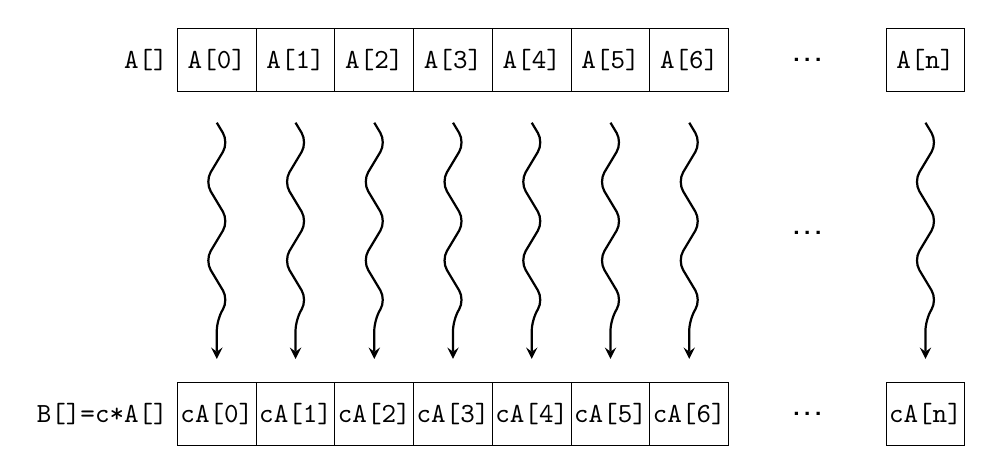
\begin{tikzpicture}
	\newcommand{\Xdisp}{0cm}
	\newcommand{\Ydisp}{0cm}
	% Array A.
	\coordinate [label=left:\texttt{A[]}] (ArrayA) at (\Xdisp,\Ydisp+0.4cm);
	\foreach \x in {0cm,1cm,2cm,3cm,4cm,5cm,6cm,9cm}
		\draw (\x, \Ydisp) rectangle (\x+1cm,\Ydisp+0.8cm);
	\foreach \x/\t in {0.5cm/A[0],1.5cm/A[1],2.5cm/A[2],3.5cm/A[3],4.5cm/A[4],5.5cm/A[5],6.5cm/A[6],9.5cm/A[n]}
		\coordinate [label=center:\texttt{\t}] (Thread\t) at (\x,\Ydisp+0.4cm);
	% Dots.
	\coordinate [label=center:\textsf{{\Large ...}}] (Dots1) at (8cm,\Ydisp+0.4cm);
	% Threads.
	\renewcommand{\Ydisp}{-0.4cm}
	\foreach \x in {0.5cm,1.5cm,2.5cm,3.5cm,4.5cm,5.5cm,6.5cm,9.5cm}
		\draw[thick, rounded corners, ->, >=stealth] (\x+0cm,\Ydisp+0cm) -- (\x+0.15cm,\Ydisp-0.25cm) -- (\x-0.15cm,\Ydisp-0.75cm) -- (\x+0.15cm,\Ydisp-1.25cm) -- (\x-0.15cm,\Ydisp-1.75cm) -- (\x+0.15cm,\Ydisp-2.25cm) -- (\x+0cm,\Ydisp-2.5cm) -- (\x+0cm,\Ydisp-3cm);
	% Dots.
	\coordinate [label=center:\textsf{{\Large ...}}] (Dots2) at (8cm,\Ydisp-1.4cm);
	% Array B.
	\renewcommand{\Ydisp}{-4.5cm}
	\coordinate [label=left:\texttt{B[]=c*A[]}] (ArrayB) at (\Xdisp,\Ydisp+0.4cm);
	\foreach \x in {0cm,1cm,2cm,3cm,4cm,5cm,6cm,9cm}
		\draw (\x, \Ydisp) rectangle (\x+1cm,\Ydisp+0.8cm);
	\foreach \x/\t in {0.5cm/cA[0],1.5cm/cA[1],2.5cm/cA[2],3.5cm/cA[3],4.5cm/cA[4],5.5cm/cA[5],6.5cm/cA[6],9.5cm/cA[n]}
		\coordinate [label=center:\texttt{\t}] (Thread\t) at (\x,\Ydisp+0.4cm);
	% Dots.
	\coordinate [label=center:\textsf{{\Large ...}}] (Dots3) at (8cm,\Ydisp+0.4cm);
\end{tikzpicture}
\caption{Data--parallelism}
\label{fig:Data-Parallelism}
\end{figure}
\subsection{GPU Programming\index{GPU!programming}}
In the GPU programming terminology CPU is referred to as \emph{host}\index{host} while GPU is called \emph{device}\index{device}. The GPU\index{GPU!memory} has its own memory separate from that of CPU's and can only work on data stored in its own memory. Any data that is to be operated on must first be copied from CPU memory into GPU memory. A special function called \emph{kernel}\index{kernel} is invoked from CPU that is run on GPU and performs its calculations. Afterwards any required result or data is copied back to CPU memory for analysis. The whole process can be summarised as:
\begin{enumerate}
	\item Allocate space for input data in CPU memory.
	\item Initialise input data.
	\item Allocate space for input data in GPU memory.
	\item Copy input data to GPU memory.
	\item Invoke kernel that runs on GPU and performs computations on input data.
	\item Copy output data back from GPU to CPU memory.
	\item Post--processing\index{post--processing} and analysis of output data on CPU.
\end{enumerate}
\section{GPU/C++ Implementation\index{C++}}
\subsection{Host (CPU) and Device (GPU) Code}
Code meant to run on CPU and GPU are compiled by different compilers; a C++ compiler and a specialised compiler provided by the GPU manufacturer to compile kernel code. The kernel code is essentially written in C with limited object--oriented capabilities and C extensions meant for interfacing with the GPU. and provide CUDA and OpenCL provide C++ interface for programming the GPU. The kernel code is stored in a separate file with .cu or .cl extension indicating the programming API (CUDA or OpenCL).

nVidia's CUDA compiler is capable of handling most C++ directives including classes and templates and can act as a standalone compiler when writing GPU applications. In case of OpenCL, any C++ compiler can be used where the GPU compiler is called from within as an OpenCL function call.
\subsection{Object--Oriented Design and Class Methods}
An object--oriented approach\index{object--oriented} requires dividing the problem into modules and sub--tasks that can be implemented as methods. Class definitions of 1D DNG implementation in CUDA and 2D DNG in OpenCL are given in appendix \ref{App:1D-DNG-Class-Definition-CUDA} and \ref{App:2D-DNG-Class-Definition-OpenCL}, respectively. The different class methods are explained in this sections.
\subsubsection{Array Allocation and Indexing}
Space for 2D or 3D array can be allocated as a 1D array where amount of space allocated is equal to product of dimensions of array. Position of an element in 1D array is a function of dimensions and indices. For example, space for a 3D array with dimensions \texttt{I}, \texttt{J} and \texttt{K} can be allocated as
\lstset{language=[ISO]C++, commentstyle=\color{green!50!black}, keywordstyle=\color{blue}, stringstyle=\color{red!60!black}}
\label{lst:3D-Array-Allocation}\index{array!allocation}
\begin{lstlisting}[caption={3D array allocation}]
int *Array3D;
Array3D = new int[I*J*K];
\end{lstlisting}
Index \texttt{(i,j,k)} can be accessed as
\label{lst:3D-Array-Access}\index{array!access}
\begin{lstlisting}[caption={Accessing elements of 3D array}]
int Value = Array3D[i+(j*I)+(k*I*J)];
\end{lstlisting}
\subsubsection{Using Macros for Array Indexing\index{macro}}
Macros make it easier to write equations and also increases readability of code.
\label{lst:Array-Access-Macro}
\begin{lstlisting}[caption={Macro to access array elements}]
#define Hy(i,j,n) Hy_[(i)+IHy*(j)+IHy*JHy*(n)]
#define am0(i,j) am0_[(i)+IHx*(j)]
#define PsiEzY(i,j) PsiEzY_[(i)+IEz*(j)]
\end{lstlisting}
\subsubsection{Constant Member Initialisation}
The constructor\index{constructor} initialises constant data members. The constructor can take some simulation parameters when the object is created. These parameters are optional and will be initialised with default values if the input fields are left empty. Some of the  basic parameters are simulation size, choice of source and interval between saving field data. The field data saved to hard disk is referred to as a snapshot\index{field snapshot}.
\subsubsection{\texttt{AllocateMemoryCPU()}}
On host, electric and magnetic fields are dynamically allocated according to size of the simulation. In addition, permittivity, permeability, Drude and PML parameters are defined for each node. These are pre--initialised before simulation to save computation time.
\subsubsection{\texttt{InitialiseCPU()}}
Field arrays, permittivity, permeability, Drude and PML parameter arrays are initialised on host.
\subsubsection{\texttt{InitialiseCL()}}
This is only for OpenCL. It first searches for a suitable device which can be CPU or GPU. OpenCL provides CPU emulation in case a GPU is not present. This is useful for debugging purposes.
\label{lst:OpenCL-Device-Search}
\begin{lstlisting}[caption={Device selection in OpenCL}]
devices = new cl_device_id[deviceListSize/sizeof(cl_device_id)];
SafeCall(!devices, "Error: No devices found.");
SafeCall(clGetContextInfo(context, CL_CONTEXT_DEVICES, deviceListSize, devices, NULL), "Error: Getting Context Info (device list, clGetContextInfo)");
\end{lstlisting}
\subsubsection{\texttt{AllocateMemoryGPU()} and \texttt{CopyDataCPUtoGPU()}}
Space is allocated for data arrays on the GPU device and data arrays initialised on host are copied onto GPU. GPU should have enough memory to store the data arrays otherwise an error will be returned. In case of CUDA this is done explicitly with \texttt{cudaMalloc()} followed by \texttt{cudaMemcpy()}. On OpenCL special data exchange buffers of type \verb|cl_mem| are created that are associated with host pointers. Data transfer from host to device is implicit in this case.
\label{lst:CUDA-Host-Memory-Allocation}
\begin{lstlisting}[caption={Device memory allocation in CUDA}]
checkCudaErrors(cudaMalloc((void **)&d_Ex_, sizeof(PRECISION)*Size*3));
checkCudaErrors(cudaMalloc((void **)&d_Hy_, sizeof(PRECISION)*Size*3));
\end{lstlisting}
\label{lst:OpenCL-Device-Memory-Buffers}
\begin{lstlisting}[caption={Device memory allocation in OpenCL}]
d_Ez_ = clCreateBuffer(context, CL_MEM_READ_WRITE | CL_MEM_USE_HOST_PTR, sizeof(PRECISION)*IEz*JEz*3, Ez_, &status);
SafeCall(status, "Error: clCreateBuffer() cannot creae input buffer for Ex_");
d_ee_ = clCreateBuffer(context, CL_MEM_READ_WRITE | CL_MEM_USE_HOST_PTR, sizeof(PRECISION)*IHx*JHx, ee_, &status);
SafeCall(status, "Error: clCreateBuffer() cannot creae input buffer for ee");
\end{lstlisting}
\subsubsection{\texttt{InitialiseCLKernelsGPU()}\index{kernel!OpenCL!initialisation}}
OpenCL implementation needs to associate all the kernels defined in the .cl file with their respective handles. These handles are variables that are used to call kernel from host. The .cl code file is loaded and compiled\index{kernel!OpenCL!compilation} first. Errors and warnings in kernel code are output on console if kernel compiler is unsuccessful in building the program. Kernel arguments\index{kernel!OpenCL!arguments} must be specified before a kernel launch. This will bind the OpenCL memory buffers for data exchange between host and device.
\label{lst:OpenCL-Setting-Kernel-Arguments}
\begin{lstlisting}[caption={Setting kernel arguments in OpenCL}]
SafeCall(clSetKernelArg(DryRun_kernel_M, 30, sizeof(cl_mem), (void *)&d_By_), "Error: Setting kernel argument d_By_");
SafeCall(clSetKernelArg(DryRun_kernel_M, 31, sizeof(cl_mem), (void *)&d_PsiEzX_), "Error: Setting kernel argument d_PsiEzX_");
\end{lstlisting}
\subsubsection{\texttt{DryRun()}\index{dry run} and \texttt{Simulation()}}
A dry run is meant to record incident fields in the absence of an obstacle or scatterer\index{scatterer}. Transmitted fields in the presence of scatterer are recorded in actual simulation. Incident and transmitted fields are used to calculate the transmission\index{coefficient!transmission ($\tau$)} and reflection\index{coefficient!reflection ($\Gamma$)} coefficients. The simulation function call takes an optional boolean argument to specify if field snapshots should be saved to hard disk.
\subsubsection{\texttt{CompleteRun()}}
A complete run method for CPU or GPU is meant to encapsulate all the underlying function calls and provide a higher level abstraction. This takes care of memory allocation, initialisation and clean--up.
\subsection{Device Kernels\index{kernel!call}}
It is necessary to synchronise all the threads calculating magnetic field before electric field calculation. Therefore, for each time step there are two kernel calls, one for magnetic and one for electric field computation. The ABC for 1D simulation requires threads at end--points to be synchronised. This is achieved in CUDA kernel with a \verb|__synchrnoizeThreads()|\index{thread synchronisation!CUDA} directive while in OpenCL the equivalent function is \verb|barrier()|\index{thread synchronisation!OpenCL}.

In CUDA, kernels are invoked\index{kernel!invocation} with a special directive wrapped in \verb|<<< >>>| while in OpenCL kernels are called by their respective handles. Examples of CUDA and OpenCL kernel invocations are given below. CUDA and OpenCL kernel code of 1D and 2D DNG simulations is given in appendices \ref{App:CUDA-1D-DNG-Kernels} and \ref{App:OpenCL-2D-DNG-Kernels}, respectively.
\label{lst:CUDA-Kernel-Call}
\begin{lstlisting}[caption={CUDA Kernel Call}]
FDTD1DDNGKernel_Simulation_E <ThreadsX, ThreadsY> <<<Blocks, Threads>>>(
					Size,
					PulseWidth,
					td,
					SourceLocation,
					SourceChoice,
					e0,
					u0,
					dt,
					dz,
					Sc,
					f,
					fp,
					dr,
					d_Ex_, d_Dx_, d_Hy_, d_By_,
					d_einf, d_uinf, d_wpesq, d_wpmsq, d_ge, d_gm,
					d_ae0, d_ae, d_be, d_ce, d_de, d_ee,
					d_am0, d_am, d_bm, d_cm, d_dm, d_em,
					d_Ext, d_Extt, d_Exz1, d_Exz2,
					x1, Z1, Z2,
					n,
					np,
					n0,
					nf);
\end{lstlisting}
\label{lst:OpenCL-Kernel-Call}
\begin{lstlisting}[caption={OpenCL Kernel Call}]
status = clEnqueueNDRangeKernel(
					commandQueue,
					Simulation_kernel_M,
					2,
					NULL,
					globalThreads,
					localThreads,
					0,
					NULL,
					&events[0]);
\end{lstlisting}
\section{Results}

\section{Performance Analysis}
\subsection{Hardware and Software Set--up}
Matlab, C++, CUDA and OpenCL implementations are tested with respect to space, time and space--time. Operating system, platform/configuration and compiler/toolchain for these implementations are listed in table \ref{Tab:OS-Platform/Configuration-Compiler/Toolchain-for-Testing}. Simulations use \verb|double| data type for arrays on 64 bit optimised platform. The CPU is an Intel Core 2 Duo E8400 @3.00 GHz with 4 GB RAM. For CUDA simulations, GPU is GTX 500 Ti with 192 shaders and 1 GB of memory. Visual C++ 2010 Express is the IDE used on 64 bit Windows 7. The flavour of linux is Fedora 14 64 bit. Hardware and software configuration is listed in table \ref{Tab:Hardware-Software-Configuration-for-Testing}.
\begin{table}[H]
\begin{center}
\vspace{0.3cm}
	\begin{tabular}{cccc}
	\hline \hline
		\rule{0pt}{2.6ex} & \multirow{2}{*}{\textbf{OS}} & \textbf{Platform/} & \textbf{Compiler/}\\
		& & \textbf{Configuration} & \textbf{Toolchain}\\
		\hline
		Matlab \rule{0pt}{2.6ex} & win, linux & x64 & NA\\
		C++ & win, cygwin, linux & x64/O3 & VC++, gcc/g++\\
		OpenCL & win, linux & x64/O3 & VC++, gcc/g++\\
		CUDA & win, linux & x64/O3 & nvcc for win/linux\\
	\hline \hline
	\end{tabular}
\end{center}
\caption{Operating system, platform/configuration and compiler/toolchain used for performance testing}
\label{Tab:OS-Platform/Configuration-Compiler/Toolchain-for-Testing}
\end{table}
\begin{table}[H]
\begin{center}
\vspace{0.3cm}
	\begin{tabular}{ll}
	\hline \hline
		\textbf{CPU} \rule{0pt}{2.6ex}& Intel Core 2 Duo E8400 @3.00 GHz\\
		\textbf{RAM} & 4.00 GB DDR2\\
		\textbf{GPU} & nVidia Geforce GTX 550 Ti 1 GB\\
		\textbf{Matlab} & 2010a 64 bit\\
		\textbf{Linux} & Fedora 14 64 bit\\
		\textbf{Windows} & Win7 64 bit\\
		\textbf{Cygwin} & 64 bit on Win7\\
	\hline \hline
	\end{tabular}
\end{center}
\caption{Hardware and software used for performance testing}
\label{Tab:Hardware-Software-Configuration-for-Testing}
\end{table}
\subsection{Spatial Performance Analysis}
Spatial performance of different CPU and GPU configurations are analysed in this section. The number of time steps are kept constant and size of simulation domain is increased. Time taken by each configuration is recorded. The data is presented with the help of graphs. Typical performances for 1D and 2D simulations are listed in tables \ref{Tab:Performance-1D-space-65536-elements} and \ref{Tab:Performance-2D-space-1024^2-elements}.
\begin{table}[H]
\begin{center}
\vspace{0.3cm}
	\begin{tabular}{cccc}
	\hline \hline
		\rule{0pt}{2.6ex} & \multirow{2}{*}{\textbf{OS}} & \multirow{2}{*}{\textbf{CPU/GPU}}  & \textbf{Time}\\
		& &  & \textbf{taken (s)}\\
		\hline
		Matlab \rule{0pt}{2.6ex} & win & CPU &19.63\\
		\hline
		\multirow{2}{*}{gcc/g++} \rule{0pt}{2.6ex} & cygwin & CPU &5.53\\
		& linux & CPU &4.6\\
		\hline
		VC++ 2010 \rule{0pt}{2.6ex} & win & CPU &5.5\\
		\hline
		\multirow{4}{*}{OpenCL} \rule{0pt}{2.6ex} & linux & CPU (GPU emulation) &22.18\\
		& win & CPU (GPU emulation) &22.9\\
		& linux & GPU &0.55\\
		& win & GPU &0.79\\
		\hline
		\multirow{2}{*}{CUDA} \rule{0pt}{2.6ex} & linux & GPU &0.46\\
		& win & GPU &1.26\\
	\hline \hline
	\end{tabular}
\end{center}
\caption{1D Spatial: Performance for array size $65536~(2^{16})$ and 1024 time steps}
\label{Tab:Performance-1D-space-65536-elements}
\end{table}
\begin{table}[H]
\begin{center}
\vspace{0.3cm}
	\begin{tabular}{cccc}
	\hline \hline
		\rule{0pt}{2.6ex} & \multirow{2}{*}{\textbf{OS}} & \multirow{2}{*}{\textbf{CPU/GPU}}  & \textbf{Time}\\
		& &  & \textbf{taken (s)}\\
		\hline
		Matlab \rule{0pt}{2.6ex} & win & CPU &361\\
		\hline
		\multirow{2}{*}{gcc/g++} \rule{0pt}{2.6ex} & cygwin & CPU &586\\
		& linux & CPU &509\\
		\hline
		VC++ 2010 \rule{0pt}{2.6ex} & win & CPU &550\\
		\hline
		\multirow{4}{*}{OpenCL} \rule{0pt}{2.6ex} & linux & CPU (GPU emulation) &39.59\\
		& win & CPU (GPU emulation) &39.33\\
		& linux & GPU &5.07\\
		& win & GPU &5.83\\
		\hline
		\multirow{2}{*}{CUDA} \rule{0pt}{2.6ex} & linux & GPU &5.33\\
		& win & GPU &6.1\\
	\hline \hline
	\end{tabular}
\end{center}
\caption{2D Spatial: Performance for array size $1024^2$ and 256 time steps}
\label{Tab:Performance-2D-space-1024^2-elements}
\end{table}
\subsubsection{1D Simulations}
\begin{figure}[H]
\centering
\begin{tikzpicture}
	\DrawAxes{size}{time~(sec)}
	\GridOn
	\TicksOn
	\XAxisText{0.0391cm/2^8}{}{}{0.625cm/2^{12}}{1.25cm/2^{13}}{2.48cm/2^{14}}{}{ 5cm/2^{15}}{10cm/2^{16}=65536}
	\YAxisText{0cm/0}{0.5cm/1.145}{1cm/2.29}{2cm/4.58}{3cm/6.87}{4cm/9.16}{5cm/11.45}{6cm/13.74}{7cm/16.03}
	\YAxisText{8cm/18.32}{9cm/20.61}{10cm/22.9}{}{}{}{}{}{}
	% 1D spatial with 1024 time steps
	\draw[line width=1.2pt,color=red!40!yellow] (0.039cm,0.16cm) -- (0.078cm,0.14cm) -- (0.16cm,0.19cm) -- (0.31cm,0.24cm) -- (0.63cm,0.44cm) -- (1.3cm,0.68cm) -- (2.5cm,1.2cm) -- (3.8cm,1.6cm) -- ( 5cm,3.4cm) -- (10cm,8.6cm);
	\draw[line width=1.2pt,color=red!10!yellow] (0.039cm,0.017cm) -- (0.078cm,0.017cm) -- (0.16cm,0.039cm) -- (0.31cm,0.061cm) -- (0.63cm,0.11cm) -- (1.3cm,0.21cm) -- (2.5cm,0.45cm) -- (3.8cm,0.66cm) -- ( 5cm,1.1cm) -- (10cm,2.4cm);
	\draw[line width=1.2pt,color=blue] (0.039cm,0.0061cm) -- (0.078cm,0.0087cm) -- (0.16cm,0.024cm) -- (0.31cm,0.044cm) -- (0.63cm,0.079cm) -- (1.3cm,0.21cm) -- (2.5cm,0.5cm) -- (3.8cm,0.75cm) -- ( 5cm, 1cm) -- (10cm, 2cm);
	\draw[line width=1.2pt,color=blue!30!white] (0.039cm,0.026cm) -- (0.078cm,0.026cm) -- (0.16cm,0.048cm) -- (0.31cm,0.066cm) -- (0.63cm,0.12cm) -- (1.3cm,0.2cm) -- (2.5cm,0.46cm) -- (3.8cm,0.57cm) -- ( 5cm,1.3cm) -- (10cm,2.4cm);
	\draw[line width=1.2pt,color=gray!70!white] (0.039cm,0.26cm) -- (0.078cm,0.28cm) -- (0.16cm,0.38cm) -- (0.31cm,0.57cm) -- (0.63cm,0.87cm) -- (1.3cm,1.4cm) -- (2.5cm,2.6cm) -- (3.8cm,3.7cm) -- ( 5cm,4.9cm) -- (10cm,9.7cm);
	\draw[line width=1.2pt,color=pink] (0.039cm,0.33cm) -- (0.078cm,0.34cm) -- (0.16cm,0.49cm) -- (0.31cm,0.56cm) -- (0.63cm,0.77cm) -- (1.3cm,1.4cm) -- (2.5cm,2.5cm) -- (3.8cm,4.9cm) -- ( 5cm,7.1cm) -- (10cm,10cm);
	\draw[line width=1.2pt,color=red!70!black] (0.039cm,0.18cm) -- (0.078cm,0.1cm) -- (0.16cm,0.1cm) -- (0.31cm,0.1cm) -- (0.63cm,0.11cm) -- (1.3cm,0.12cm) -- (2.5cm,0.14cm) -- (3.8cm,0.15cm) -- ( 5cm,0.17cm) -- (10cm,0.24cm);
	\draw[line width=1.2pt,color=red] (0.039cm,0.21cm) -- (0.078cm,0.2cm) -- (0.16cm,0.21cm) -- (0.31cm,0.21cm) -- (0.63cm,0.21cm) -- (1.3cm,0.22cm) -- (2.5cm,0.23cm) -- (3.8cm,0.26cm) -- ( 5cm,0.28cm) -- (10cm,0.34cm);
	\draw[line width=1.2pt,color=green!50!black] (0.039cm,0.045cm) -- (0.078cm,0.048cm) -- (0.16cm,0.047cm) -- (0.31cm,0.053cm) -- (0.63cm,0.062cm) -- (1.3cm,0.083cm) -- (2.5cm,0.1cm) -- (3.8cm,0.12cm) -- ( 5cm,0.12cm) -- (10cm,0.2cm);
	\draw[line width=1.2pt,color=green] (0.039cm,0.39cm) -- (0.078cm,0.38cm) -- (0.16cm,0.36cm) -- (0.31cm,0.37cm) -- (0.63cm,0.36cm) -- (1.3cm,0.39cm) -- (2.5cm,0.41cm) -- (3.8cm,0.45cm) -- ( 5cm,0.46cm) -- (10cm,0.55cm);
	\DrawLegend
\end{tikzpicture}
\caption{1D Spatial: General performance comparison}
\label{fig:Performance-1D-space}
\end{figure}
\begin{figure}[H]
\centering
\begin{tikzpicture}
	\DrawAxes{size}{time~(sec)}
	\GridOn
	\TicksOn
	\XAxisText{0.313cm/2^8}{0.625cm/2^{9}}{1.25cm/2^{10}}{2.5cm/2^{11}}{ 5cm/2^{12}(4096)}{10cm/2^{13}(8192)}{}{}{}{}{}
	\YAxisText{0.00cm/0.00}{0.50cm/0.16}{1.00cm/0.32}{1.50cm/0.48}{2.00cm/0.64}{2.50cm/0.80}{3.00cm/0.96}{3.50cm/1.12}{4.00cm/1.28}
	\YAxisText{4.50cm/1.44}{5.00cm/1.60}{5.50cm/1.76}{6.00cm/1.92}{6.50cm/2.08}{7.00cm/2.24}{7.50cm/2.40}{8.00cm/2.56}{8.50cm/2.72}
	\YAxisText{9.00cm/2.88}{9.50cm/3.04}{10.00cm/3.20}{}{}{}{}{}{}
	% 1D spatial upto size=2^13 with 1024 time steps
	\draw[line width=1.2pt,color=red!40!yellow] (0.31cm,1.1cm) -- (0.63cm, 1cm) -- (1.3cm,1.4cm) -- (2.5cm,1.7cm) -- ( 5cm,3.1cm) -- (10cm,4.9cm);
	\draw[line width=1.2pt,color=red!10!yellow] (0.31cm,0.13cm) -- (0.63cm,0.13cm) -- (1.3cm,0.28cm) -- (2.5cm,0.44cm) -- ( 5cm,0.78cm) -- (10cm,1.5cm);
	\draw[line width=1.2pt,color=blue] (0.31cm,0.044cm) -- (0.63cm,0.063cm) -- (1.3cm,0.17cm) -- (2.5cm,0.31cm) -- ( 5cm,0.56cm) -- (10cm,1.5cm);
	\draw[line width=1.2pt,color=blue!30!white] (0.31cm,0.19cm) -- (0.63cm,0.19cm) -- (1.3cm,0.34cm) -- (2.5cm,0.47cm) -- ( 5cm,0.84cm) -- (10cm,1.4cm);
	\draw[line width=1.2pt,color=gray!70!white] (0.31cm,1.9cm) -- (0.63cm, 2cm) -- (1.3cm,2.8cm) -- (2.5cm,4.1cm) -- ( 5cm,6.3cm) -- (10cm,10cm);
	\draw[line width=1.2pt,color=pink] (0.31cm,2.3cm) -- (0.63cm,2.4cm) -- (1.3cm,3.5cm) -- (2.5cm, 4cm) -- ( 5cm,5.5cm) -- (10cm,9.7cm);
	\draw[line width=1.2pt,color=red!70!black] (0.31cm,1.3cm) -- (0.63cm,0.72cm) -- (1.3cm,0.73cm) -- (2.5cm,0.74cm) -- ( 5cm,0.77cm) -- (10cm,0.84cm);
	\draw[line width=1.2pt,color=red] (0.31cm,1.5cm) -- (0.63cm,1.4cm) -- (1.3cm,1.5cm) -- (2.5cm,1.5cm) -- ( 5cm,1.5cm) -- (10cm,1.6cm);
	\draw[line width=1.2pt,color=green!50!black] (0.31cm,0.32cm) -- (0.63cm,0.34cm) -- (1.3cm,0.34cm) -- (2.5cm,0.38cm) -- ( 5cm,0.45cm) -- (10cm,0.59cm);
	\draw[line width=1.2pt,color=green] (0.31cm,2.8cm) -- (0.63cm,2.7cm) -- (1.3cm,2.6cm) -- (2.5cm,2.6cm) -- ( 5cm,2.6cm) -- (10cm,2.8cm);
	\DrawLegend
\end{tikzpicture}
\caption{1D Spatial: Performance for smaller array sizes}
\label{fig:Performance-smaller-array-1D-space}
\end{figure}
\begin{figure}[H]
\centering
\begin{tikzpicture}
	\DrawAxes{size}{time~(sec)}
	\GridOn
	\TicksOn
	\XAxisText{0.00122cm/2^8}{}{}{0.625cm/2^{17}}{1.25cm/2^{18}}{2.5cm/2^{19}}{ 5cm/2^{20}}{10cm/2^{21}}{}{}{}{}
	\YAxisText{0cm/0}{ 1cm/18}{ 2cm/36}{ 3cm/54}{ 4cm/72}{ 5cm/90}{ 6cm/108}{ 7cm/126}{ 8cm/144}
	\YAxisText{}{ 9cm/162}{10cm/180}{}{}{}{}{}{}
	% 1D spatial extended with 1024 time steps
	\draw[line width=1.2pt,color=blue] (0.0012cm,0.00078cm) -- (0.0024cm,0.0011cm) -- (0.0049cm,0.0031cm) -- (0.0098cm,0.0056cm) -- (0.02cm,0.01cm) -- (0.039cm,0.027cm) -- (0.078cm,0.064cm) -- (0.12cm,0.095cm) -- (0.16cm,0.13cm) -- (0.31cm,0.26cm) -- (0.63cm,0.54cm) -- (1.3cm,1.1cm) -- (2.5cm,2.2cm) -- ( 5cm,4.4cm) -- (10cm,8.8cm);
	\draw[line width=1.2pt,color=blue!30!white] (0.0012cm,0.0033cm) -- (0.0024cm,0.0033cm) -- (0.0049cm,0.0061cm) -- (0.0098cm,0.0083cm) -- (0.02cm,0.015cm) -- (0.039cm,0.026cm) -- (0.078cm,0.059cm) -- (0.12cm,0.073cm) -- (0.16cm,0.17cm) -- (0.31cm,0.3cm) -- (0.63cm,0.62cm) -- (1.3cm,1.3cm) -- (2.5cm,2.5cm) -- ( 5cm, 5cm) -- (10cm,10cm);
	\draw[line width=1.2pt,color=red!70!black] (0.0012cm,0.023cm) -- (0.0024cm,0.013cm) -- (0.0049cm,0.013cm) -- (0.0098cm,0.013cm) -- (0.02cm,0.014cm) -- (0.039cm,0.015cm) -- (0.078cm,0.017cm) -- (0.12cm,0.019cm) -- (0.16cm,0.022cm) -- (0.31cm,0.031cm) -- (0.63cm,0.049cm) -- (1.3cm,0.086cm) -- (2.5cm,0.16cm) -- ( 5cm,0.3cm) -- (10cm,0.59cm);
	\draw[line width=1.2pt,color=red] (0.0012cm,0.027cm) -- (0.0024cm,0.026cm) -- (0.0049cm,0.026cm) -- (0.0098cm,0.027cm) -- (0.02cm,0.027cm) -- (0.039cm,0.028cm) -- (0.078cm,0.029cm) -- (0.12cm,0.033cm) -- (0.16cm,0.035cm) -- (0.31cm,0.044cm) -- (0.63cm,0.063cm) -- (1.3cm,0.098cm) -- (2.5cm,0.17cm) -- ( 5cm,0.3cm) -- (10cm,0.63cm);
	\draw[line width=1.2pt,color=green!50!black] (0.0012cm,0.0057cm) -- (0.0024cm,0.0061cm) -- (0.0049cm,0.006cm) -- (0.0098cm,0.0068cm) -- (0.02cm,0.0079cm) -- (0.039cm,0.011cm) -- (0.078cm,0.013cm) -- (0.12cm,0.016cm) -- (0.16cm,0.016cm) -- (0.31cm,0.026cm) -- (0.63cm,0.046cm) -- (1.3cm,0.084cm) -- (2.5cm,0.16cm) -- ( 5cm,0.32cm) -- (10cm,0.63cm);
	\draw[line width=1.2pt,color=green] (0.0012cm,0.05cm) -- (0.0024cm,0.048cm) -- (0.0049cm,0.046cm) -- (0.0098cm,0.047cm) -- (0.02cm,0.046cm) -- (0.039cm,0.05cm) -- (0.078cm,0.052cm) -- (0.12cm,0.057cm) -- (0.16cm,0.059cm) -- (0.31cm,0.07cm) -- (0.63cm,0.097cm) -- (1.3cm,0.13cm) -- (2.5cm,0.21cm) -- ( 5cm,0.35cm) -- (10cm,0.73cm);
	\DrawLegendNoMatlabandOpenCLEmu
\end{tikzpicture}
\caption{1D Spatial: Extended tests}
\label{fig:Performance-1D-space-Extended}
\end{figure}
\begin{figure}[H]
\centering
\begin{tikzpicture}
	\DrawAxes{size}{time~(sec)}
	\GridOn
	\TicksOn
	\XAxisText{0.00122cm/2^8}{}{}{0.625cm/2^{17}}{1.25cm/2^{18}}{2.5cm/2^{19}}{ 5cm/2^{20}}{10cm/2^{21}}{}{}{}{}
	\YAxisText{0cm/0}{ 1cm/1.4}{ 2cm/2.8}{ 3cm/4.2}{ 4cm/5.6}{ 5cm/7.0}{ 6cm/8.4}{ 7cm/9.8}{ 8cm/11.2}
	\YAxisText{}{ 9cm/12.6}{10cm/14.0}{}{}{}{}{}{}
	% 1D spatial GPU comparison 1024 time steps
	\draw[line width=1.2pt,color=red!70!black] (0.0012cm,0.29cm) -- (0.0024cm,0.16cm) -- (0.0049cm,0.17cm) -- (0.0098cm,0.17cm) -- (0.02cm,0.18cm) -- (0.039cm,0.19cm) -- (0.078cm,0.22cm) -- (0.12cm,0.25cm) -- (0.16cm,0.28cm) -- (0.31cm,0.39cm) -- (0.63cm,0.64cm) -- (1.3cm,1.1cm) -- (2.5cm, 2cm) -- ( 5cm,3.9cm) -- (10cm,7.6cm);
	\draw[line width=1.2pt,color=red] (0.0012cm,0.34cm) -- (0.0024cm,0.33cm) -- (0.0049cm,0.34cm) -- (0.0098cm,0.34cm) -- (0.02cm,0.34cm) -- (0.039cm,0.36cm) -- (0.078cm,0.38cm) -- (0.12cm,0.42cm) -- (0.16cm,0.45cm) -- (0.31cm,0.56cm) -- (0.63cm,0.81cm) -- (1.3cm,1.3cm) -- (2.5cm,2.2cm) -- ( 5cm,3.9cm) -- (10cm, 8cm);
	\draw[line width=1.2pt,color=green!50!black] (0.0012cm,0.073cm) -- (0.0024cm,0.078cm) -- (0.0049cm,0.077cm) -- (0.0098cm,0.087cm) -- (0.02cm,0.1cm) -- (0.039cm,0.14cm) -- (0.078cm,0.17cm) -- (0.12cm,0.2cm) -- (0.16cm,0.2cm) -- (0.31cm,0.33cm) -- (0.63cm,0.59cm) -- (1.3cm,1.1cm) -- (2.5cm,2.1cm) -- ( 5cm,4.1cm) -- (10cm,8.2cm);
	\draw[line width=1.2pt,color=green] (0.0012cm,0.64cm) -- (0.0024cm,0.61cm) -- (0.0049cm,0.59cm) -- (0.0098cm,0.6cm) -- (0.02cm,0.59cm) -- (0.039cm,0.64cm) -- (0.078cm,0.67cm) -- (0.12cm,0.74cm) -- (0.16cm,0.76cm) -- (0.31cm,0.9cm) -- (0.63cm,1.2cm) -- (1.3cm,1.7cm) -- (2.5cm,2.7cm) -- ( 5cm,4.5cm) -- (10cm,9.4cm);
	\DrawLegendGPU
\end{tikzpicture}
\caption{1D Spatial: GPU comparison}
\label{fig:GPU-comparison-1D-space}
\end{figure}

\subsubsection{2D Simulations}
\begin{figure}[H]
\centering
\begin{tikzpicture}
	\DrawAxes{size}{time~(sec)}
	\GridOn
	\TicksOn
	\XAxisText{0.313cm/32^2}{1.25cm/128^2}{2.5cm/256^2}{3.75cm/384^2}{ 5cm/512^2}{6.25cm/640^2}{7.5cm/768^2}{8.75cm/896^2}{10cm/1024^2}
	\YAxisText{0.00cm/0}{1.00cm/60}{2.00cm/120}{3.00cm/180}{4.00cm/240}{5.00cm/300}{6.00cm/360}{7.00cm/420}{8.00cm/480}
	\YAxisText{9.00cm/540}{10.00cm/600}{}{}{}{}{}{}{}
	% 2D spatial all plots with 256 time steps
	\draw[line width=1.2pt,color=red!40!yellow] (0.31cm,0.019cm) -- (0.63cm,0.025cm) -- (1.3cm,0.048cm) -- (2.5cm,0.2cm) -- (3.8cm,0.59cm) -- ( 5cm,1.2cm) -- (6.3cm,2.1cm) -- (7.5cm,3.3cm) -- (8.8cm,4.4cm) -- (10cm, 6cm);
	\draw[line width=1.2pt,color=red!10!yellow] (0.31cm,0.00082cm) -- (0.63cm,0.0038cm) -- (1.3cm,0.02cm) -- (2.5cm,0.3cm) -- (3.8cm,0.41cm) -- ( 5cm,2.5cm) -- (6.3cm,2.5cm) -- (7.5cm,5.2cm) -- (8.8cm,5.9cm) -- (10cm,9.8cm);
	\draw[line width=1.2pt,color=blue] (0.31cm,0.00087cm) -- (0.63cm,0.0033cm) -- (1.3cm,0.017cm) -- (2.5cm,0.32cm) -- (3.8cm,0.5cm) -- ( 5cm,2.1cm) -- (6.3cm,2.7cm) -- (7.5cm,4.4cm) -- (8.8cm,5.6cm) -- (10cm,8.5cm);
	\draw[line width=1.2pt,color=blue!30!white] (0.31cm,0.0032cm) -- (0.63cm,0.0062cm) -- (1.3cm,0.022cm) -- (2.5cm,0.13cm) -- (3.8cm,0.37cm) -- ( 5cm,2.3cm) -- (6.3cm,2.3cm) -- (7.5cm,4.8cm) -- (8.8cm,5.4cm) -- (10cm,9.2cm);
	\draw[line width=1.2pt,color=gray!70!white] (0.31cm,0.0093cm) -- (0.63cm,0.011cm) -- (1.3cm,0.017cm) -- (2.5cm,0.049cm) -- (3.8cm,0.091cm) -- ( 5cm,0.17cm) -- (6.3cm,0.24cm) -- (7.5cm,0.36cm) -- (8.8cm,0.5cm) -- (10cm,0.66cm);
	\draw[line width=1.2pt,color=pink] (0.31cm,0.013cm) -- (0.63cm,0.013cm) -- (1.3cm,0.017cm) -- (2.5cm,0.046cm) -- (3.8cm,0.095cm) -- ( 5cm,0.18cm) -- (6.3cm,0.25cm) -- (7.5cm,0.36cm) -- (8.8cm,0.45cm) -- (10cm,0.66cm);
	\draw[line width=1.2pt,color=red!70!black] (0.31cm,0.0022cm) -- (0.63cm,0.0027cm) -- (1.3cm,0.0035cm) -- (2.5cm,0.0078cm) -- (3.8cm,0.014cm) -- ( 5cm,0.023cm) -- (6.3cm,0.034cm) -- (7.5cm,0.049cm) -- (8.8cm,0.066cm) -- (10cm,0.085cm);
	\draw[line width=1.2pt,color=red] (0.31cm,0.0067cm) -- (0.63cm,0.0067cm) -- (1.3cm,0.0078cm) -- (2.5cm,0.012cm) -- (3.8cm,0.02cm) -- ( 5cm,0.03cm) -- (6.3cm,0.043cm) -- (7.5cm,0.058cm) -- (8.8cm,0.075cm) -- (10cm,0.097cm);
	\draw[line width=1.2pt,color=green!50!black] (0.31cm,0.0012cm) -- (0.63cm,0.0014cm) -- (1.3cm,0.0021cm) -- (2.5cm,0.0068cm) -- (3.8cm,0.013cm) -- ( 5cm,0.024cm) -- (6.3cm,0.035cm) -- (7.5cm,0.051cm) -- (8.8cm,0.068cm) -- (10cm,0.089cm);
	\draw[line width=1.2pt,color=green] (0.31cm,0.005cm) -- (0.63cm,0.005cm) -- (1.3cm,0.0067cm) -- (2.5cm,0.011cm) -- (3.8cm,0.019cm) -- ( 5cm,0.03cm) -- (6.3cm,0.043cm) -- (7.5cm,0.06cm) -- (8.8cm,0.081cm) -- (10cm,0.1cm);
	\DrawLegend
\end{tikzpicture}
\caption{2D Spatial: General performance comparison}
\label{fig:Performance-2D-space}
\end{figure}
\begin{figure}[H]
\centering
\begin{tikzpicture}
	\DrawAxes{size}{time~(sec)}
	\GridOn
	\TicksOn
	\XAxisText{0.833cm/32^2}{1.67cm/64^2}{3.33cm/128^2}{6.67cm/256^2}{10cm/384^2}{}{}{}{}
	\YAxisText{0.00cm/0.0}{1.00cm/3.6}{2.00cm/7.2}{3.00cm/10.8}{4.00cm/14.4}{5.00cm/18.0}{6.00cm/21.6}{7.00cm/25.2}{8.00cm/28.8}
	\YAxisText{9.00cm/32.4}{10.00cm/36.0}{}{}{}{}{}{}{}
	% 2D spatial small sizes with 256 time steps
	\draw[line width=1.2pt,color=red!40!yellow] (0.83cm,0.32cm) -- (1.7cm,0.42cm) -- (3.3cm,0.8cm) -- (6.7cm,3.3cm) -- (10cm,9.9cm);
	\draw[line width=1.2pt,color=red!10!yellow] (0.83cm,0.014cm) -- (1.7cm,0.064cm) -- (3.3cm,0.33cm) -- (6.7cm, 5cm) -- (10cm,6.8cm);
	\draw[line width=1.2pt,color=blue] (0.83cm,0.014cm) -- (1.7cm,0.054cm) -- (3.3cm,0.29cm) -- (6.7cm,5.3cm) -- (10cm,8.4cm);
	\draw[line width=1.2pt,color=blue!30!white] (0.83cm,0.053cm) -- (1.7cm,0.1cm) -- (3.3cm,0.36cm) -- (6.7cm,2.1cm) -- (10cm,6.2cm);
	\draw[line width=1.2pt,color=gray!70!white] (0.83cm,0.16cm) -- (1.7cm,0.19cm) -- (3.3cm,0.28cm) -- (6.7cm,0.81cm) -- (10cm,1.5cm);
	\draw[line width=1.2pt,color=pink] (0.83cm,0.21cm) -- (1.7cm,0.21cm) -- (3.3cm,0.29cm) -- (6.7cm,0.77cm) -- (10cm,1.6cm);
	\draw[line width=1.2pt,color=red!70!black] (0.83cm,0.036cm) -- (1.7cm,0.044cm) -- (3.3cm,0.058cm) -- (6.7cm,0.13cm) -- (10cm,0.23cm);
	\draw[line width=1.2pt,color=red] (0.83cm,0.11cm) -- (1.7cm,0.11cm) -- (3.3cm,0.13cm) -- (6.7cm,0.19cm) -- (10cm,0.33cm);
	\draw[line width=1.2pt,color=green!50!black] (0.83cm,0.02cm) -- (1.7cm,0.023cm) -- (3.3cm,0.036cm) -- (6.7cm,0.11cm) -- (10cm,0.22cm);
	\draw[line width=1.2pt,color=green] (0.83cm,0.083cm) -- (1.7cm,0.083cm) -- (3.3cm,0.11cm) -- (6.7cm,0.18cm) -- (10cm,0.32cm);
	\DrawLegend
\end{tikzpicture}
\caption{2D Spatial: Performance for smaller array sizes}
\label{fig:Performance-smaller-array-2D-space}
\end{figure}
\begin{figure}[H]
\centering
\begin{tikzpicture}
	\DrawAxes{size}{time~(sec)}
	\GridOn
	\TicksOn
	\XAxisText{0.192cm/32^2}{0.769cm/128^2}{1.54cm/256^2}{2.31cm/384^2}{3.08cm/512^2}{3.85cm/640^2}{4.62cm/768^2}{5.38cm/896^2}{6.15cm/1024^2}
	\XAxisText{}{7.69cm/1280^2}{}{}{10cm/1664^2}{}{}{}{}{}
	\YAxisText{0.00cm/0}{1.00cm/10}{2.00cm/20}{3.00cm/30}{4.00cm/40}{5.00cm/50}{6.00cm/60}{7.00cm/70}{8.00cm/80}
	\YAxisText{}{9.00cm/90}{10.00cm/100}{}{}{}{}{}{}
	% 2D spatial extended plots with 256 time steps
	\draw[line width=1.2pt,color=gray!70!white] (0.19cm,0.056cm) -- (0.38cm,0.068cm) -- (0.77cm,0.1cm) -- (1.5cm,0.29cm) -- (2.3cm,0.55cm) -- (3.1cm, 1cm) -- (3.8cm,1.4cm) -- (4.6cm,2.2cm) -- (5.4cm, 3cm) -- (6.2cm, 4cm) -- (6.9cm,4.7cm) -- (7.7cm,5.9cm) -- (8.5cm,7.2cm) -- (9.2cm,9.2cm) -- (10cm,9.9cm);
	\draw[line width=1.2pt,color=pink] (0.19cm,0.075cm) -- (0.38cm,0.076cm) -- (0.77cm,0.1cm) -- (1.5cm,0.28cm) -- (2.3cm,0.57cm) -- (3.1cm,1.1cm) -- (3.8cm,1.5cm) -- (4.6cm,2.2cm) -- (5.4cm,2.7cm) -- (6.2cm,3.9cm) -- (6.9cm,4.6cm) -- (7.7cm,5.8cm) -- (8.5cm,6.6cm) -- (9.2cm,8.8cm) -- (10cm,9.4cm);
	\draw[line width=1.2pt,color=red!70!black] (0.19cm,0.013cm) -- (0.38cm,0.016cm) -- (0.77cm,0.021cm) -- (1.5cm,0.047cm) -- (2.3cm,0.083cm) -- (3.1cm,0.14cm) -- (3.8cm,0.21cm) -- (4.6cm,0.29cm) -- (5.4cm,0.39cm) -- (6.2cm,0.51cm) -- (6.9cm,0.64cm) -- (7.7cm,0.79cm) -- (8.5cm,0.96cm) -- (9.2cm,1.2cm) -- (10cm,1.4cm);
	\draw[line width=1.2pt,color=red] (0.19cm,0.04cm) -- (0.38cm,0.04cm) -- (0.77cm,0.047cm) -- (1.5cm,0.07cm) -- (2.3cm,0.12cm) -- (3.1cm,0.18cm) -- (3.8cm,0.26cm) -- (4.6cm,0.34cm) -- (5.4cm,0.45cm) -- (6.2cm,0.58cm) -- (6.9cm,0.73cm) -- (7.7cm,0.93cm) -- (8.5cm,1.1cm) -- (9.2cm,1.3cm);
	\draw[line width=1.2pt,color=green!50!black] (0.19cm,0.0071cm) -- (0.38cm,0.0081cm) -- (0.77cm,0.013cm) -- (1.5cm,0.041cm) -- (2.3cm,0.08cm) -- (3.1cm,0.14cm) -- (3.8cm,0.21cm) -- (4.6cm,0.3cm) -- (5.4cm,0.41cm) -- (6.2cm,0.53cm) -- (6.9cm,0.68cm) -- (7.7cm,0.83cm) -- (8.5cm, 1cm) -- (9.2cm,1.2cm) -- (10cm,1.5cm);
	\draw[line width=1.2pt,color=green] (0.19cm,0.03cm) -- (0.38cm,0.03cm) -- (0.77cm,0.04cm) -- (1.5cm,0.066cm) -- (2.3cm,0.12cm) -- (3.1cm,0.18cm) -- (3.8cm,0.26cm) -- (4.6cm,0.36cm) -- (5.4cm,0.48cm) -- (6.2cm,0.61cm) -- (6.9cm,0.76cm) -- (7.7cm,0.94cm) -- (8.5cm,1.2cm) -- (9.2cm,1.4cm);
	\DrawLegendNoMatlabandVCGCC
\end{tikzpicture}
\caption{2D Spatial: Extended tests}
\label{fig:Performance-2D-space-Extended}
\end{figure}
\begin{figure}[H]
\centering
\begin{tikzpicture}
	\DrawAxes{size}{time~(sec)}
	\GridOn
	\TicksOn
	\XAxisText{0.192cm/32^2}{0.769cm/128^2}{1.54cm/256^2}{2.31cm/384^2}{3.08cm/512^2}{3.85cm/640^2}{4.62cm/768^2}{5.38cm/896^2}{6.15cm/1024^2}
	\XAxisText{}{7.69cm/1280^2}{}{}{10cm/1664^2}{}{}{}{}{}
	\YAxisText{0.00cm/0.0}{1.00cm/1.5}{2.00cm/3.0}{3.00cm/4.5}{4.00cm/6.0}{5.00cm/7.5}{6.00cm/9.0}{7.00cm/10.5}{8.00cm/12.0}
	\YAxisText{}{9.00cm/13.5}{10.00cm/15.0}{}{}{}{}{}{}
	% 2D spatial GPU comparison with 256 time steps
	\draw[line width=1.2pt,color=red!70!black] (0.19cm,0.087cm) -- (0.38cm,0.11cm) -- (0.77cm,0.14cm) -- (1.5cm,0.31cm) -- (2.3cm,0.55cm) -- (3.1cm,0.93cm) -- (3.8cm,1.4cm) -- (4.6cm,1.9cm) -- (5.4cm,2.6cm) -- (6.2cm,3.4cm) -- (6.9cm,4.3cm) -- (7.7cm,5.3cm) -- (8.5cm,6.4cm) -- (9.2cm,7.8cm) -- (10cm,9.2cm);
	\draw[line width=1.2pt,color=red] (0.19cm,0.27cm) -- (0.38cm,0.27cm) -- (0.77cm,0.31cm) -- (1.5cm,0.47cm) -- (2.3cm,0.79cm) -- (3.1cm,1.2cm) -- (3.8cm,1.7cm) -- (4.6cm,2.3cm) -- (5.4cm, 3cm) -- (6.2cm,3.9cm) -- (6.9cm,4.9cm) -- (7.7cm,6.2cm) -- (8.5cm,7.3cm) -- (9.2cm,8.7cm);
	\draw[line width=1.2pt,color=green!50!black] (0.19cm,0.047cm) -- (0.38cm,0.054cm) -- (0.77cm,0.085cm) -- (1.5cm,0.27cm) -- (2.3cm,0.53cm) -- (3.1cm,0.94cm) -- (3.8cm,1.4cm) -- (4.6cm, 2cm) -- (5.4cm,2.7cm) -- (6.2cm,3.6cm) -- (6.9cm,4.5cm) -- (7.7cm,5.5cm) -- (8.5cm,6.7cm) -- (9.2cm,8.1cm) -- (10cm,9.7cm);
	\draw[line width=1.2pt,color=green] (0.19cm,0.2cm) -- (0.38cm,0.2cm) -- (0.77cm,0.27cm) -- (1.5cm,0.44cm) -- (2.3cm,0.77cm) -- (3.1cm,1.2cm) -- (3.8cm,1.7cm) -- (4.6cm,2.4cm) -- (5.4cm,3.2cm) -- (6.2cm,4.1cm) -- (6.9cm,5.1cm) -- (7.7cm,6.3cm) -- (8.5cm,7.7cm) -- (9.2cm,9.1cm);
	\DrawLegendGPU
\end{tikzpicture}
\caption{2D Spatial: GPU comparison}
\label{fig:GPU-comparison-2D-space}
\end{figure}
\newpage
\subsection{Temporal Performance Analysis}
This section presents performance analysis graphs with respect to total number of time steps. The simulation size is kept constant for both 1D and 2D cases and number of time steps are progressively increased. In 1D simulations, size is set at 65536 elements, whereas, in 2D simulations size is $512^2$ elements.
\begin{table}[H]
\begin{center}
\vspace{0.3cm}
	\begin{tabular}{cccc}
	\hline \hline
		\rule{0pt}{2.6ex} & \multirow{2}{*}{\textbf{OS}} & \multirow{2}{*}{\textbf{CPU/GPU}}  & \textbf{Time}\\
		& &  & \textbf{taken (s)}\\
		\hline
		Matlab \rule{0pt}{2.6ex} & win & CPU &158.31\\
		\hline
		\multirow{2}{*}{gcc/g++} \rule{0pt}{2.6ex} & cygwin & CPU &62.41\\
		& linux & CPU &34.94\\
		\hline
		VC++ 2010 \rule{0pt}{2.6ex} & win & CPU &51.35\\
		\hline
		\multirow{4}{*}{OpenCL} \rule{0pt}{2.6ex} & linux & CPU (GPU emulation) &351\\
		& win & CPU (GPU emulation) &408\\
		& linux & GPU &4.06\\
		& win & GPU &6.46\\
		\hline
		\multirow{2}{*}{CUDA} \rule{0pt}{2.6ex} & linux & GPU &3.66\\
		& win & GPU &5.16\\
	\hline \hline
	\end{tabular}
\end{center}
\caption{1D Temporal: Performance for array size 65536 and 10000 time steps}
\label{Tab:Performance-1D-time-10000-steps}
\end{table}
\begin{table}[H]
\begin{center}
\vspace{0.3cm}
	\begin{tabular}{cccc}
	\hline \hline
		\rule{0pt}{2.6ex} & \multirow{2}{*}{\textbf{OS}} & \multirow{2}{*}{\textbf{CPU/GPU}}  & \textbf{Time}\\
		& &  & \textbf{taken (s)}\\
		\hline
		Matlab \rule{0pt}{2.6ex} & win & CPU &1271 (21.2 min.)\\
		\hline
		\multirow{2}{*}{gcc/g++} \rule{0pt}{2.6ex} & cygwin & CPU &2800 (46.7 min.)\\
		& linux & CPU &1765 (29.4 min.)\\
		\hline
		VC++ 2010 \rule{0pt}{2.6ex} & win & CPU &2594 (43.2 min.)\\
		\hline
		\multirow{4}{*}{OpenCL} \rule{0pt}{2.6ex} & linux & CPU (GPU emulation) &148.771\\
		& win & CPU (GPU emulation) &162.89\\
		& linux & GPU &12.028\\
		& win & GPU &13.91\\
		\hline
		\multirow{2}{*}{CUDA} \rule{0pt}{2.6ex} & linux & GPU &13.06\\
		& win & GPU &14.246\\
	\hline \hline
	\end{tabular}
\end{center}
\caption{2D Temporal: Performance for array size $512^2$ and 5000 time steps}
\label{Tab:Performance-2D-time-5000-steps}
\end{table}
\subsubsection{1D Simulations}
\begin{figure}[H]
\centering
\begin{tikzpicture}
	\DrawAxes{steps}{time~(sec)}
	\GridOn
	\TicksOn
	\XAxisText{0.1cm/100}{1cm/1000}{2cm/2000}{3cm/3000}{4cm/4000}{5cm/5000}{6cm/6000}{7cm/7000}{8cm/8000}
	\XAxisText{9cm/9000}{10cm/10000}{}{}{}{}{}{}{}
	\YAxisText{0.00cm/0}{1.00cm/41}{2.00cm/82}{3.00cm/123}{4.00cm/164}{5.00cm/205}{6.00cm/246}{7.00cm/287}{8.00cm/328}
	\YAxisText{9.00cm/369}{10.00cm/410}{}{}{}{}{}{}{}
	% ------- 1D temporal with 65536 size -------
	\draw[line width=1.2pt,color=red!40!yellow] (0.1cm,0.041cm) -- (0.25cm,0.096cm) -- (0.5cm,0.18cm) -- ( 1cm,0.36cm) -- (1.5cm,0.55cm) -- ( 2cm,0.73cm) -- (2.5cm,0.94cm) -- ( 3cm,1.1cm) -- (3.5cm,1.3cm) -- ( 4cm,1.6cm) -- (4.5cm,1.7cm) -- ( 5cm,1.9cm) -- ( 6cm,2.3cm) -- ( 7cm,2.6cm) -- ( 8cm,3.2cm) -- ( 9cm,3.5cm) -- (10cm,3.9cm);
	\draw[line width=1.2pt,color=red!10!yellow] (0.1cm,0.013cm) -- (0.25cm,0.037cm) -- (0.5cm,0.068cm) -- ( 1cm,0.13cm) -- (1.5cm,0.19cm) -- ( 2cm,0.28cm) -- (2.5cm,0.33cm) -- ( 3cm,0.4cm) -- (3.5cm,0.47cm) -- ( 4cm,0.55cm) -- (4.5cm,0.62cm) -- ( 5cm,0.7cm) -- ( 6cm,0.84cm) -- ( 7cm,1.1cm) -- ( 8cm,1.2cm) -- ( 9cm,1.4cm) -- (10cm,1.5cm);
	\draw[line width=1.2pt,color=blue] (0.1cm,0.012cm) -- (0.25cm,0.022cm) -- (0.5cm,0.043cm) -- ( 1cm,0.084cm) -- (1.5cm,0.13cm) -- ( 2cm,0.18cm) -- (2.5cm,0.22cm) -- ( 3cm,0.25cm) -- (3.5cm,0.3cm) -- ( 4cm,0.34cm) -- (4.5cm,0.41cm) -- ( 5cm,0.43cm) -- ( 6cm,0.51cm) -- ( 7cm,0.62cm) -- ( 8cm,0.68cm) -- ( 9cm,0.82cm) -- (10cm,0.85cm);
	\draw[line width=1.2pt,color=blue!30!white] (0.1cm,0.013cm) -- (0.25cm,0.031cm) -- (0.5cm,0.066cm) -- ( 1cm,0.14cm) -- (1.5cm,0.19cm) -- ( 2cm,0.27cm) -- (2.5cm,0.31cm) -- ( 3cm,0.37cm) -- (3.5cm,0.44cm) -- ( 4cm,0.51cm) -- (4.5cm,0.58cm) -- ( 5cm,0.63cm) -- ( 6cm,0.75cm) -- ( 7cm,0.89cm) -- ( 8cm, 1cm) -- ( 9cm,1.2cm) -- (10cm,1.3cm);
	\draw[line width=1.2pt,color=gray!70!white] (0.1cm,0.072cm) -- (0.25cm,0.17cm) -- (0.5cm,0.47cm) -- ( 1cm,0.67cm) -- (1.5cm, 1cm) -- ( 2cm,1.7cm) -- (2.5cm,2.1cm) -- ( 3cm, 2cm) -- (3.5cm,2.3cm) -- ( 4cm,3.5cm) -- (4.5cm,3.9cm) -- ( 5cm,3.3cm) -- ( 6cm,5.7cm) -- ( 7cm,6.2cm) -- ( 8cm,5.5cm) -- ( 9cm,6.1cm) -- (10cm,8.6cm);
	\draw[line width=1.2pt,color=pink] (0.1cm,0.11cm) -- (0.25cm,0.25cm) -- (0.5cm,0.5cm) -- ( 1cm, 1cm) -- (1.5cm,1.5cm) -- ( 2cm, 2cm) -- (2.5cm,2.5cm) -- ( 3cm, 3cm) -- (3.5cm,3.6cm) -- ( 4cm,4.3cm) -- (4.5cm,4.7cm) -- ( 5cm, 5cm) -- ( 6cm, 6cm) -- ( 7cm, 7cm) -- ( 8cm, 8cm) -- ( 9cm, 9cm) -- (10cm,10cm);
	\draw[line width=1.2pt,color=red!70!black] (0.1cm,0.0042cm) -- (0.25cm,0.004cm) -- (0.5cm,0.0064cm) -- ( 1cm,0.011cm) -- (1.5cm,0.016cm) -- ( 2cm,0.021cm) -- (2.5cm,0.026cm) -- ( 3cm,0.031cm) -- (3.5cm,0.036cm) -- ( 4cm,0.041cm) -- (4.5cm,0.045cm) -- ( 5cm,0.05cm) -- ( 6cm,0.061cm) -- ( 7cm,0.07cm) -- ( 8cm,0.079cm) -- ( 9cm,0.089cm) -- (10cm,0.099cm);
	\draw[line width=1.2pt,color=red] (0.1cm,0.004cm) -- (0.25cm,0.0066cm) -- (0.5cm,0.01cm) -- ( 1cm,0.018cm) -- (1.5cm,0.025cm) -- ( 2cm,0.034cm) -- (2.5cm,0.041cm) -- ( 3cm,0.048cm) -- (3.5cm,0.056cm) -- ( 4cm,0.062cm) -- (4.5cm,0.07cm) -- ( 5cm,0.079cm) -- ( 6cm,0.093cm) -- ( 7cm,0.11cm) -- ( 8cm,0.12cm) -- ( 9cm,0.14cm) -- (10cm,0.16cm);
	\draw[line width=1.2pt,color=green!50!black] (0.1cm,0.0037cm) -- (0.25cm,0.004cm) -- (0.5cm,0.0062cm) -- ( 1cm,0.011cm) -- (1.5cm,0.015cm) -- ( 2cm,0.019cm) -- (2.5cm,0.024cm) -- ( 3cm,0.028cm) -- (3.5cm,0.032cm) -- ( 4cm,0.037cm) -- (4.5cm,0.041cm) -- ( 5cm,0.046cm) -- ( 6cm,0.054cm) -- ( 7cm,0.063cm) -- ( 8cm,0.072cm) -- ( 9cm,0.081cm) -- (10cm,0.089cm);
	\draw[line width=1.2pt,color=green] (0.1cm,0.009cm) -- (0.25cm,0.0058cm) -- (0.5cm,0.0091cm) -- ( 1cm,0.015cm) -- (1.5cm,0.021cm) -- ( 2cm,0.027cm) -- (2.5cm,0.033cm) -- ( 3cm,0.04cm) -- (3.5cm,0.046cm) -- ( 4cm,0.052cm) -- (4.5cm,0.059cm) -- ( 5cm,0.064cm) -- ( 6cm,0.077cm) -- ( 7cm,0.089cm) -- ( 8cm,0.1cm) -- ( 9cm,0.11cm) -- (10cm,0.13cm);
	\DrawLegend
\end{tikzpicture}
\caption{1D Temporal: General performance comparison}
\label{fig:Performance-1D-time}
\end{figure}
\begin{figure}[H]
\centering
\begin{tikzpicture}
	\DrawAxes{steps}{time~(sec)}
	\GridOn
	\TicksOn
	\XAxisText{1cm/100}{2.5cm/250}{5cm/500}{10cm/1000}{}{}{}{}{}
	\YAxisText{0.00cm/0.0}{0.50cm/2.1}{1.00cm/4.2}{1.50cm/6.3}{2.00cm/8.4}{2.50cm/10.5}{3.00cm/12.6}{3.50cm/14.7}{4.00cm/16.8}	
	\YAxisText{4.50cm/18.9}{5.00cm/21.0}{5.50cm/23.1}{6.00cm/25.2}{6.50cm/27.3}{7.00cm/29.4}{7.50cm/31.5}{8.00cm/33.6}{8.50cm/35.7}
	\YAxisText{9.00cm/37.8}{9.50cm/39.9}{10.00cm/42.0}{}{}{}{}{}{}
	% ------- 1D temporal for shorter simulations -------
	\draw[line width=1.2pt,color=red!40!yellow] ( 1cm,0.4cm) -- (2.5cm,0.94cm) -- ( 5cm,1.8cm) -- (10cm,3.5cm);
	\draw[line width=1.2pt,color=red!10!yellow] ( 1cm,0.13cm) -- (2.5cm,0.36cm) -- ( 5cm,0.66cm) -- (10cm,1.3cm);
	\draw[line width=1.2pt,color=blue] ( 1cm,0.11cm) -- (2.5cm,0.21cm) -- ( 5cm,0.42cm) -- (10cm,0.82cm);
	\draw[line width=1.2pt,color=blue!30!white] ( 1cm,0.13cm) -- (2.5cm,0.3cm) -- ( 5cm,0.65cm) -- (10cm,1.3cm);
	\draw[line width=1.2pt,color=gray!70!white] ( 1cm,0.7cm) -- (2.5cm,1.7cm) -- ( 5cm,4.5cm) -- (10cm,6.6cm);
	\draw[line width=1.2pt,color=pink] ( 1cm, 1cm) -- (2.5cm,2.5cm) -- ( 5cm,4.9cm) -- (10cm,9.9cm);
	\draw[line width=1.2pt,color=red!70!black] ( 1cm,0.041cm) -- (2.5cm,0.039cm) -- ( 5cm,0.063cm) -- (10cm,0.11cm);
	\draw[line width=1.2pt,color=red] ( 1cm,0.039cm) -- (2.5cm,0.065cm) -- ( 5cm,0.1cm) -- (10cm,0.18cm);
	\draw[line width=1.2pt,color=green!50!black] ( 1cm,0.036cm) -- (2.5cm,0.039cm) -- ( 5cm,0.06cm) -- (10cm,0.1cm);
	\draw[line width=1.2pt,color=green] ( 1cm,0.088cm) -- (2.5cm,0.057cm) -- ( 5cm,0.089cm) -- (10cm,0.15cm);
	\DrawLegend
\end{tikzpicture}
\caption{1D Temporal: Performance for shorter simulations}
\label{fig:Performance-shorter-times-1D-time}
\end{figure}
\begin{figure}[H]
\centering
\begin{tikzpicture}
	\DrawAxes{steps}{time~(sec)}
	\GridOn
	\TicksOn
	\XAxisText{0.1cm/100}{1cm/1000}{2cm/2000}{3cm/3000}{4cm/4000}{5cm/5000}{6cm/6000}{7cm/7000}{8cm/8000}
	\XAxisText{9cm/9000}{10cm/10000}{}{}{}{}{}{}{}
	\YAxisText{0.00cm/0}{1.00cm/6}{2.00cm/12}{3.00cm/18}{4.00cm/24}{5.00cm/30}{6.00cm/36}{7.00cm/42}{8.00cm/48}
	\YAxisText{9.00cm/54}{10.00cm/60}{}{}{}{}{}{}{}
	% ------- 1D temporal comparison with VC++ -------
	\draw[line width=1.2pt,color=red!40!yellow] (0.1cm,0.28cm) -- (0.25cm,0.66cm) -- (0.5cm,1.3cm) -- ( 1cm,2.5cm) -- (1.5cm,3.8cm) -- ( 2cm, 5cm) -- (2.5cm,6.4cm) -- ( 3cm,7.8cm) -- (3.5cm,9.1cm);
	\draw[line width=1.2pt,color=red!10!yellow] (0.1cm,0.09cm) -- (0.25cm,0.25cm) -- (0.5cm,0.46cm) -- ( 1cm,0.9cm) -- (1.5cm,1.3cm) -- ( 2cm,1.9cm) -- (2.5cm,2.3cm) -- ( 3cm,2.7cm) -- (3.5cm,3.2cm) -- ( 4cm,3.8cm) -- (4.5cm,4.2cm) -- ( 5cm,4.8cm) -- ( 6cm,5.7cm) -- ( 7cm,7.2cm) -- ( 8cm,8.1cm) -- ( 9cm,9.3cm);
	\draw[line width=1.2pt,color=blue] (0.1cm,0.079cm) -- (0.25cm,0.15cm) -- (0.5cm,0.3cm) -- ( 1cm,0.58cm) -- (1.5cm,0.87cm) -- ( 2cm,1.2cm) -- (2.5cm,1.5cm) -- ( 3cm,1.7cm) -- (3.5cm, 2cm) -- ( 4cm,2.3cm) -- (4.5cm,2.8cm) -- ( 5cm,2.9cm) -- ( 6cm,3.5cm) -- ( 7cm,4.2cm) -- ( 8cm,4.6cm) -- ( 9cm,5.6cm) -- (10cm,5.8cm);
	\draw[line width=1.2pt,color=blue!30!white] (0.1cm,0.092cm) -- (0.25cm,0.21cm) -- (0.5cm,0.45cm) -- ( 1cm,0.94cm) -- (1.5cm,1.3cm) -- ( 2cm,1.9cm) -- (2.5cm,2.1cm) -- ( 3cm,2.6cm) -- (3.5cm, 3cm) -- ( 4cm,3.5cm) -- (4.5cm,3.9cm) -- ( 5cm,4.3cm) -- ( 6cm,5.2cm) -- ( 7cm,6.1cm) -- ( 8cm, 7cm) -- ( 9cm,7.9cm) -- (10cm,8.6cm);
	\draw[line width=1.2pt,color=gray!70!white] (0.1cm,0.49cm) -- (0.25cm,1.2cm) -- (0.5cm,3.2cm) -- ( 1cm,4.6cm) -- (1.5cm, 7cm);
	\draw[line width=1.2pt,color=pink] (0.1cm,0.73cm) -- (0.25cm,1.7cm) -- (0.5cm,3.4cm) -- ( 1cm,6.9cm);
	\draw[line width=1.2pt,color=red!70!black] (0.1cm,0.029cm) -- (0.25cm,0.027cm) -- (0.5cm,0.044cm) -- ( 1cm,0.077cm) -- (1.5cm,0.11cm) -- ( 2cm,0.14cm) -- (2.5cm,0.18cm) -- ( 3cm,0.21cm) -- (3.5cm,0.24cm) -- ( 4cm,0.28cm) -- (4.5cm,0.31cm) -- ( 5cm,0.34cm) -- ( 6cm,0.41cm) -- ( 7cm,0.48cm) -- ( 8cm,0.54cm) -- ( 9cm,0.61cm) -- (10cm,0.68cm);
	\draw[line width=1.2pt,color=red] (0.1cm,0.028cm) -- (0.25cm,0.045cm) -- (0.5cm,0.071cm) -- ( 1cm,0.13cm) -- (1.5cm,0.17cm) -- ( 2cm,0.23cm) -- (2.5cm,0.28cm) -- ( 3cm,0.33cm) -- (3.5cm,0.38cm) -- ( 4cm,0.43cm) -- (4.5cm,0.48cm) -- ( 5cm,0.54cm) -- ( 6cm,0.63cm) -- ( 7cm,0.74cm) -- ( 8cm,0.85cm) -- ( 9cm,0.96cm) -- (10cm,1.1cm);
	\draw[line width=1.2pt,color=green!50!black] (0.1cm,0.025cm) -- (0.25cm,0.027cm) -- (0.5cm,0.042cm) -- ( 1cm,0.072cm) -- (1.5cm,0.1cm) -- ( 2cm,0.13cm) -- (2.5cm,0.16cm) -- ( 3cm,0.19cm) -- (3.5cm,0.22cm) -- ( 4cm,0.25cm) -- (4.5cm,0.28cm) -- ( 5cm,0.31cm) -- ( 6cm,0.37cm) -- ( 7cm,0.43cm) -- ( 8cm,0.49cm) -- ( 9cm,0.55cm) -- (10cm,0.61cm);
	\draw[line width=1.2pt,color=green] (0.1cm,0.062cm) -- (0.25cm,0.04cm) -- (0.5cm,0.062cm) -- ( 1cm,0.1cm) -- (1.5cm,0.14cm) -- ( 2cm,0.19cm) -- (2.5cm,0.23cm) -- ( 3cm,0.27cm) -- (3.5cm,0.31cm) -- ( 4cm,0.36cm) -- (4.5cm,0.4cm) -- ( 5cm,0.44cm) -- ( 6cm,0.52cm) -- ( 7cm,0.61cm) -- ( 8cm,0.7cm) -- ( 9cm,0.78cm) -- (10cm,0.86cm);
	\DrawLegend
\end{tikzpicture}
\caption{1D Temporal: Performance comparison with respect to VC++}
\label{fig:Performance-wrtVC++-1D-time}
\end{figure}
\begin{figure}[H]
\centering
\begin{tikzpicture}
	\DrawAxes{steps}{time~(sec)}
	\GridOn
	\TicksOn
	\XAxisText{0.1cm/100}{1cm/1000}{2cm/2000}{3cm/3000}{4cm/4000}{5cm/5000}{6cm/6000}{7cm/7000}{8cm/8000}
	\XAxisText{9cm/9000}{10cm/10000}{}{}{}{}{}{}{}
	\YAxisText{0.00cm/0}{1.00cm/1}{2.00cm/2}{3.00cm/3}{4.00cm/4}{5.00cm/5}{6.00cm/6}{7.00cm/7}{8.00cm/8}
	\YAxisText{9.00cm/9}{10.00cm/10}{}{}{}{}{}{}{}
	% ------- 1D temporal GPU comparison -------
	\draw[line width=1.2pt,color=red!40!yellow] (0.1cm,1.7cm) -- (0.25cm, 4cm) -- (0.5cm,7.6cm);
	\draw[line width=1.2pt,color=red!10!yellow] (0.1cm,0.54cm) -- (0.25cm,1.5cm) -- (0.5cm,2.8cm) -- ( 1cm,5.4cm) -- (1.5cm,7.9cm);
	\draw[line width=1.2pt,color=blue] (0.1cm,0.48cm) -- (0.25cm,0.89cm) -- (0.5cm,1.8cm) -- ( 1cm,3.5cm) -- (1.5cm,5.2cm) -- ( 2cm,7.2cm) -- (2.5cm, 9cm);
	\draw[line width=1.2pt,color=blue!30!white] (0.1cm,0.55cm) -- (0.25cm,1.3cm) -- (0.5cm,2.7cm) -- ( 1cm,5.6cm) -- (1.5cm, 8cm);
	\draw[line width=1.2pt,color=gray!70!white] (0.1cm,2.9cm) -- (0.25cm,7.1cm);
	\draw[line width=1.2pt,color=pink] (0.1cm,4.4cm) -- (0.25cm,10cm);
	\draw[line width=1.2pt,color=red!70!black] (0.1cm,0.17cm) -- (0.25cm,0.16cm) -- (0.5cm,0.26cm) -- ( 1cm,0.46cm) -- (1.5cm,0.66cm) -- ( 2cm,0.86cm) -- (2.5cm,1.1cm) -- ( 3cm,1.3cm) -- (3.5cm,1.5cm) -- ( 4cm,1.7cm) -- (4.5cm,1.9cm) -- ( 5cm,2.1cm) -- ( 6cm,2.5cm) -- ( 7cm,2.9cm) -- ( 8cm,3.3cm) -- ( 9cm,3.7cm) -- (10cm,4.1cm);
	\draw[line width=1.2pt,color=red] (0.1cm,0.17cm) -- (0.25cm,0.27cm) -- (0.5cm,0.43cm) -- ( 1cm,0.75cm) -- (1.5cm, 1cm) -- ( 2cm,1.4cm) -- (2.5cm,1.7cm) -- ( 3cm, 2cm) -- (3.5cm,2.3cm) -- ( 4cm,2.6cm) -- (4.5cm,2.9cm) -- ( 5cm,3.2cm) -- ( 6cm,3.8cm) -- ( 7cm,4.4cm) -- ( 8cm,5.1cm) -- ( 9cm,5.8cm) -- (10cm,6.5cm);
	\draw[line width=1.2pt,color=green!50!black] (0.1cm,0.15cm) -- (0.25cm,0.16cm) -- (0.5cm,0.25cm) -- ( 1cm,0.43cm) -- (1.5cm,0.61cm) -- ( 2cm,0.79cm) -- (2.5cm,0.97cm) -- ( 3cm,1.2cm) -- (3.5cm,1.3cm) -- ( 4cm,1.5cm) -- (4.5cm,1.7cm) -- ( 5cm,1.9cm) -- ( 6cm,2.2cm) -- ( 7cm,2.6cm) -- ( 8cm,2.9cm) -- ( 9cm,3.3cm) -- (10cm,3.7cm);
	\draw[line width=1.2pt,color=green] (0.1cm,0.37cm) -- (0.25cm,0.24cm) -- (0.5cm,0.37cm) -- ( 1cm,0.63cm) -- (1.5cm,0.86cm) -- ( 2cm,1.1cm) -- (2.5cm,1.4cm) -- ( 3cm,1.6cm) -- (3.5cm,1.9cm) -- ( 4cm,2.1cm) -- (4.5cm,2.4cm) -- ( 5cm,2.6cm) -- ( 6cm,3.1cm) -- ( 7cm,3.7cm) -- ( 8cm,4.2cm) -- ( 9cm,4.7cm) -- (10cm,5.2cm);
	\DrawLegend
\end{tikzpicture}
\caption{1D Temporal: GPU comparison}
\label{fig:GPU-comparison-1D-time}
\end{figure}
\subsubsection{2D Simulations}

% GPU Implementation
\chapter{GPU implementation}
\section{GPU Specifications}
\section{API Selection}
\section{Simulation Parameters}
\section{Memory Considerations}
\section{Thread Management}

% Conclusion
\chapter{Conclusion}
The goal of this thesis was accelerated GPU implementation of lossless cylindrical cloak. It was shown that materials with negative permeability and permittivity can be effectively modelled using Drude dispersive model. The numerical results showed good agreement with theoretical values in the case of DNG slab problem. The lossy results showed an interesting prospect that DNG medium might act as an absorbing layer similar to PML due to its complete absorption of higher frequency waves.

The 1D and 2D cases of slab problem was then implemented using C++ and GPU. A comprehensive performance analysis showed that GPU was able to perform much better both, as the problem domain and maximum time stepping are increased. For smaller problems, however, it is better to use Matlab or C++ due to data copying overhead associated with GPU implementation.

The lossless case of cylindrical cloak, as presented by Zhao et. al. in \cite{Radial-Zhao}, was implemented using Matlab, C++ and finally on GPU with minor modifications. The simulations showed adequate similarity to accepted results.

% Bibliography
\nocite{*}
\bibliographystyle{ieeetr} %plain, ieeetr
\bibliography{FDTDRef}

\appendix
\chapter{FDTD Code for 1D Wave Propagation in Free Space}
\begin{lstlisting}
% Simulation parameters.
SIZE = 512; % No. of spatial steps
MaxTime = 512; % No. of time steps
PulseWidth = 128; % Width of Gaussian Pulse
imp0 = 377.0; % Impedence of free space

% Constants.
c = 3e8;
pi = 3.141592654;
e0 = (1e-9)/(36*pi);
u0 = (1e-7)*4*pi;

dt = 1e-12;
dz = 3e-4;
Sc = c * dt/dz

% Initialization.
Ex = zeros ( SIZE, MaxTime ); % z-component of E-field
Hy = zeros ( SIZE, MaxTime ); % y-component of H-field
PLOT1(1) = 0; % Data for plotting.

% Outer loop for time-stepping.
tic
for q = 2:MaxTime
    % Calculation of Hy using update difference equation for Hy. This is time step q.
    Hy(1:SIZE-1,q) = Hy(1:SIZE-1,q-1) + ( ( Ex(1:SIZE-1,q-1) - Ex(2:SIZE,q-1) ) * dt/(u0*dz) );
    % ABC for H at SIZE.
    Hy(SIZE,q) = Hy(SIZE-1,q-1) + (Sc-1)/(Sc+1)*(Hy(SIZE-1,q) - Hy(SIZE,q-1) );
    
    % Calculation of Ez using updated difference equation for Ez. This is time step q+1/2.
    Ex(2:SIZE,q) = Ex(2:SIZE, q-1) + ( dt/(e0*dz)*(Hy(1:SIZE-1, q) - Hy(2:SIZE, q)) );
    % ABC for E at 1.
    Ex(1,q) = Ex(2,q-1) + (Sc-1)/(Sc+1)*(Ex(2,q) - Ex(2,q-1));
    
    % Activating a plane-wave source.
    Ex(100,q) = Ex(100,q) + exp( -1*(q-PulseWidth)^2/PulseWidth ) * Sc;
end
toc

% Simulation animation.
for i=1:MaxTime
    figure (2)
    plot ( Ex(:,i) )
end

\end{lstlisting}

\chapter{1D FDTD Demonstrating CBC}
\begin{lstlisting}
% Simulation parameters.
SIZE = 1024; % No. of spatial steps
MaxTime = 2024; % No. of time steps
imp0 = 377.0; % Impedence of free space

% Constants.
c = 3e8;
pi = 3.141592654;
e0 = (1e-9)/(36*pi);
u0 = (1e-7)*4*pi;

dt = 0.8e-12;
dx = 3e-4;
Sc = c * dt/dx

% Initialization.
Ez = zeros ( SIZE, MaxTime ); % z-component of E-field
Hy = zeros ( SIZE, MaxTime ); % y-component of H-field
PLOT1(1) = 0; % Data for plotting.

% Outer loop for time-stepping.
tic
for q = 2:MaxTime
    % Calculation of Hy using update difference equation for Hy. This is time step q.
    Hy(1:SIZE-1,q) = Hy(1:SIZE-1,q-1) + ( ( Ez(2:SIZE,q-1) - Ez(1:SIZE-1,q-1) ) * dt/(u0*dx) );
    % CBC for H at SIZE.
    Hy(SIZE,q) = Hy(SIZE,q-1) + ( ( Ez(1,q-1) - Ez(SIZE,q-1) ) * dt/(u0*dx) );
    
    % Calculation of Ez using updated difference equation for Ez. This is time step q+1/2.
    Ez(2:SIZE,q) = Ez(2:SIZE, q-1) + ( dt/(e0*dx)*(Hy(2:SIZE, q) - Hy(1:SIZE-1, q)) );
    % CBC for E at 1.
    Ez(1,q) = Ez(1,q-1) + ( dt/(e0*dx)*(Hy(1, q) - Hy(SIZE, q)) );
    
    % Activating a plane-wave source.
    Ez(100,q) = Ez(100,q) + exp( -1*((q-256)^2)/1000 ) * Sc;
end
toc

% Simulation animation.
for i=1:MaxTime
    figure (2)
    plot ( Ez(:,i) )
end

\end{lstlisting}

\end{document}




